%%%%%%%%%%%%%%%%%%%%%%%%%%%%%%%%%%%%%%%%%
%
% http://users.ecs.soton.ac.uk/srg/softwaretools/document/templates/
% and¯¯
% Sunil Patel
% http://www.sunilpatel.co.uk/thesis-template/
%
% License:
% CC BY-NC-SA 3.0 (http://creativecommons.org/licenses/by-nc-sa/3.0/)
%
% Note:
% Make sure to edit document variables in the Thesis.cls file
%
%%%%%%%%%%%%%%%%%%%%%%%%%%%%%%%%%%%%%%%%%

%----------------------------------------------------------------------------------------
%	PACKAGES AND OTHER DOCUMENT CONFIGURATIONS
%----------------------------------------------------------------------------------------
\documentclass[11pt, oneside]{Thesis} % The default font size and one-sided printing (no margin offsets)
\graphicspath{{Pictures/}{Pictures/balancedcorrelationcharts/}{Pictures/unbalancedcorrelationcharts/}{Pictures/Chapter2/}{Pictures/Chapter4/}{Pictures/GIS/}{Pictures/Chapter3/}{Pictures/Chapter5/}} % Specifies the directory where pictures are stored
\lstset{inputpath=ListingDocuments/}
\usepackage{mathtools}
\usepackage{natbib}
\usepackage{float}
\usepackage{caption}
\usepackage{subcaption}
\usepackage{multirow}
\usepackage{eurosym}
\usepackage{longtable}
\usepackage{changepage}
\usepackage{array}
\usepackage{url}
\usepackage{graphicx}
\usepackage{algorithm}% http://ctan.org/pkg/algorithm
\usepackage{algpseudocode}% http://ctan.org/pkg/algorithmicx
\usepackage{multirow}
\usepackage[table,xcdraw]{xcolor}
\usepackage{colortbl}
\usepackage{lipsum}
\usepackage{listings}
\usepackage{verbatim}
\usepackage{amssymb}
\usepackage{commath}
\usepackage{amsmath}
\usepackage{amssymb}

\usepackage{enumitem}
\captionsetup[subfigure]{labelfont=rm}
\usepackage[table]{xcolor}
 % Use the natbib reference package - read up on this to edit the reference style; if you want text (e.g. Smith et al., 2012) for the in-text references (instead of numbers), remove 'numbers' 
\setcitestyle{authoryear}
\usepackage[export]{adjustbox}
\hypersetup{urlcolor=blue, colorlinks=true} % Colors hyperlinks in blue - change to black if annoying
\title{\ttitle} % Defines the thesis title - don't touch this
\begin{document}

\frontmatter % Use roman page numbering style (i, ii, iii, iv...) for the pre-content pages

\setstretch{1.3} % Line spacing of 1.3

% Define the page headers using the FancyHdr package and set up for one-sided printing
\fancyhead{} % Clears all page headers and footers
\rhead{\thepage} % Sets the right side header to show the page number
\lhead{} % Clears the left side page header

\pagestyle{fancy} % Finally, use the "fancy" page style to implement the FancyHdr headers

\newcommand{\HRule}{\rule{\linewidth}{0.5mm}} % New command to make the lines in the title page

% PDF meta-data
\hypersetup{pdftitle={\ttitle}}
\hypersetup{pdfsubject=\subjectname}
\hypersetup{pdfauthor=\authornames}
\hypersetup{pdfkeywords=\keywordnames}

%----------------------------------------------------------------------------------------
%	TITLE PAGE
%----------------------------------------------------------------------------------------

\begin{titlepage}
\begin{center}

\textsc{\LARGE \univname}\\[1.5cm] % University name
\textsc{\Large Masters Thesis}\\[0.5cm] % Thesis type

\HRule \\[0.4cm] % Horizontal line
{\huge \bfseries \ttitle}\\[0.4cm] % Thesis title
\HRule \\[1.5cm] % Horizontal line
 
\begin{minipage}{0.4\textwidth}
\begin{flushleft} \large
\emph{Author:}\\
{\authornames} % Author name - remove the \href bracket to remove the link
\end{flushleft}
\end{minipage}
\begin{minipage}{0.4\textwidth}
\begin{flushright} \large
\emph{Supervisor:} \\
\supname % Supervisor name - remove the \href bracket to remove the link  
\end{flushright}
\end{minipage}\\[3cm]
 
\large \textit{A thesis submitted in fulfilment of the requirements\\ for the degree of \degreename}\\[0.3cm] % University requirement text
\textit{in the}\\[0.4cm]
\facname\\\deptname\\[2cm] % Research group name and department name
 
{\large \today}\\[4cm] % Date
%\includegraphics{Logo} % University/department logo - uncomment to place it
 
\vfill
\end{center}

\end{titlepage}

%----------------------------------------------------------------------------------------
%	DECLARATION PAGE
%	Your institution may give you a different text to place here
%----------------------------------------------------------------------------------------

\Declaration{

\addtocontents{toc}{\vspace{1em}} % Add a gap in the Contents, for aesthetics

I, \authornames, declare that this thesis titled, `\ttitle' and the work presented in it are my own. I confirm that:

\begin{itemize} 
\item[\tiny{$\blacksquare$}] This work was done wholly or mainly while in candidature for a research degree at this University.
\item[\tiny{$\blacksquare$}] Where any part of this thesis has previously been submitted for a degree or any other qualification at this University or any other institution, this has been clearly stated.s
\item[\tiny{$\blacksquare$}] Where I have consulted the published work of others, this is always clearly attributed.
\item[\tiny{$\blacksquare$}] Where I have quoted from the work of others, the source is always given. With the exception of such quotations, this thesis is entirely my own work.
\item[\tiny{$\blacksquare$}] I have acknowledged all main sources of help.
\item[\tiny{$\blacksquare$}] Where the thesis is based on work done by myself jointly with others, I have made clear exactly what was done by others and what I have contributed myself.\\
\end{itemize}
 
Signed:\\
\rule[1em]{25em}{0.5pt} % This prints a line for the signature
 
Date:\\
\rule[1em]{25em}{0.5pt} % This prints a line to write the date
}

\clearpage % Start a new page

%----------------------------------------------------------------------------------------
%	QUOTATION PAGE
%----------------------------------------------------------------------------------------

\pagestyle{empty} % No headers or footers for the following pages

\null\vfill % Add some space to move the quote down the page a bit

\textit{``If we have data, let's look at data. If all we have are opinions, let's go with mine"}

\begin{flushright}
Jim Barksdale, former Netscape CEO
\end{flushright}

\vfill\vfill\vfill\vfill\vfill\vfill\null % Add some space at the bottom to position the quote just right

\clearpage % Start a new page

%----------------------------------------------------------------------------------------
%	ABSTRACT PAGE
%----------------------------------------------------------------------------------------

\addtotoc{Abstract} % Add the "Abstract" page entry to the Contents

\abstract{\addtocontents{toc}{\vspace{1em}} 
\textit{Small-medium enterprises (SMEs) play an important role in the economy 
	worldwide  and  they  normally  need  to  borrow  funds  from  financial 
	institutions.  Thus,  an  accurate  credit  risk  model  to  predict  the  probability 
	that  these  firms  might  be  bankrupt  and  cannot  pay  back  the  loans  on 
	time is very crucial.}




  
\clearpage % Start a new page


%----------------------------------------------------------------------------------------
%	ACKNOWLEDGEMENTS
%----------------------------------------------------------------------------------------

\setstretch{1.3} % Reset the line-spacing to 1.3 for body text (if it has changed)

\acknowledgements{\addtocontents{toc}{\vspace{1em}} % Add a gap in the Contents, for aesthetics

I would like to thank my supervisor, \supname , for all the help she has provided to me in this project.
}
\clearpage % Start a new page

%----------------------------------------------------------------------------------------
%	LIST OF CONTENTS/FIGURES/TABLES PAGES
%----------------------------------------------------------------------------------------

\pagestyle{fancy} % The page style headers have been "empty" all this time, now use the "fancy" headers as defined before to bring them back

\lhead{\emph{Contents}} % Set the left side page header to "Contents"
\tableofcontents % Write out the Table of Contents

\lhead{\emph{List of Figures}} % Set the left side page header to "List of Figures"
\listoffigures % Write out the List of Figures

\lhead{\emph{List of Tables}} % Set the left side page header to "List of Tables"
\listoftables % Write out the List of Tables

%----------------------------------------------------------------------------------------
%	ABBREVIATIONS
%----------------------------------------------------------------------------------------

\clearpage % Start a new page

\setstretch{1.5} % Set the line spacing to 1.5, this makes the following tables easier to read

\lhead{\emph{Abbreviations}} % Set the left side page header to "Abbreviations"
\listofsymbols{ll} % Include a list of Abbreviations (a table of two columns)
{
\textbf{ABT} & \textbf{A}nalytics \textbf{B}ase \textbf{T}able \\
\textbf{AIB} & \textbf{A}llied \textbf{I}rish \textbf{B}anks \\
\textbf{ANN} & \textbf{A}rtificial \textbf{N}eural \textbf{N}etwork\\
\textbf{API} & \textbf{A}pplication \textbf{P}rogramming \textbf{I}nterface \\
\textbf{AUC} & \textbf{A}rea \textbf{U}nder \textbf{C}urve \\

\textbf{BA} & \textbf{B}alanced \textbf{A}ccuracy \\

\textbf{CRAN} & The \textbf{C}omprehensive \textbf{R} \textbf{A}chive \textbf{N}etwork\\
\textbf{CRISP-DM} & \textbf{C}ross \textbf{I}ndustry \textbf{S}tandard \textbf{P}rocess for \textbf{D}ata \textbf{Mining} \\
\textbf{CSO} & \textbf{C}entral \textbf{S}tatistics \textbf{O}ffice \\

\textbf{ED} & \textbf{E}lectoral \textbf{D}ivision \\
\textbf{EDW} & \textbf{E}nterprise \textbf{D}ata \textbf{W}arehouse \\
\textbf{EPER} & \textbf{E}vent \textbf{P}recision \textbf{E}quals \textbf{R}ecall \\

\textbf{FN} & \textbf{F}alse \textbf{N}egative \\
\textbf{FP} & \textbf{F}alse \textbf{P}ositive \\

\textbf{GDD} & \textbf{G}eo \textbf{D}irectory \textbf{D}atabase \\
\textbf{GIS} & \textbf{G}eogrphic \textbf{I}nformation \textbf{S}ystem \\
\textbf{GPS} & \textbf{G}lobal \textbf{P}ositioning \textbf{S}ystem \\

\textbf{ID3} & \textbf{I}terative \textbf{D}ichotomiser \textbf{3} \\
\textbf{IG} & \textbf{I}nformation \textbf{G}ain \\
\textbf{IV} & \textbf{I}nformation \textbf{V}alue \\

\textbf{KDD} & \textbf{K}nowledge \textbf{D}iscovery in \textbf{D}atabases\\
\textbf{KNN} & \textbf{K} \textbf{N}earest in \textbf{N}eighbours\\
\textbf{K-S} & \textbf{K}ologorov \textbf{S}mirnov\\

\textbf{LA} & \textbf{L}ocal \textbf{A}uthority \\
\textbf{LOOCV} & \textbf{L}eave \textbf{O}ne \textbf{O}ut \textbf{C}ross \textbf{V}alidation\\

\textbf{MCC} & \textbf{M}erchant \textbf{C}ategory \textbf{C}ode \\
\textbf{MR} & \textbf{M}isclassification \textbf{R}ate \\

\textbf{OECD} & The \textbf{O}rganisation for \textbf{E}conomic \textbf{C}o-operation and \textbf{D}evelopment \\




\textbf{R} & The \textbf{R} Project for Statistical Computing\\
\textbf{ROC} & \textbf{R}eceiver \textbf{O}perating \textbf{C}haracteristic \\

\textbf{TN} & \textbf{T}rue \textbf{N}egative \\
\textbf{TP} & \textbf{T}rue \textbf{P}ositive \\

\textbf{SAS} & \textbf{S}tatistical \textbf{A}nalysis \textbf{S}ystem\\
\textbf{SME/SMEs} & \textbf{S}mall and \textbf{M}edium-sized \textbf{E}nterprises \\
\textbf{SMOTE} & \textbf{S}ynthetic \textbf{M}inority \textbf{O}versampling \textbf{T}echnique \\
\textbf{SQL} & \textbf{S}tructured \textbf{Q}uery \textbf{L}anguage \\
\textbf{SVM} & \textbf{S}upport \textbf{V}ector \textbf{M}achines \\

\textbf{WoE} & \textbf{W}eight of \textbf{E}vidence \\
}
%----------------------------------------------------------------------------------------
%	DEDICATION
%----------------------------------------------------------------------------------------

\setstretch{1.3} % Return the line spacing back to 1.3

\pagestyle{empty} % Page style needs to be empty for this page

\dedicatory{For/Dedicated to/To my\ldots} % Dedication text

\addtocontents{toc}{\vspace{2em}} % Add a gap in the Contents, for aesthetics

%----------------------------------------------------------------------------------------
%	THESIS CONTENT - CHAPTERS
%----------------------------------------------------------------------------------------

\mainmatter % Begin numeric (1,2,3...) page numbering

\pagestyle{fancy} % Return the page headers back to the "fancy" style

% Include the chapters of the thesis as separate files from the Chapters folder
% Uncomment the lines as you write the chapters

% Chapter Template

\chapter{Introduction} % Main chapter title

\label{Chapter1} % Change X to a consecutive number; for referencing this chapter elsewhere, use \ref{ChapterX}

\lhead{Chapter 1. \emph{Introduction}} % Change X to a consecutive number; this is for the header on each page - perhaps a shortened title

% INTRO
\section*{Overview of Project Area}

In the finance credit risk is one of the oldest forms of risk. Credit risk can be defined as one party ``a lender'' trusting another party ``a borrower'' enough that they are happy to give them with money ``some credit'' where they anticipate to be paid back not instantly but after some time interval, the credit risk is the probability or chance that the ``lender'' is never paid back by the ``borrower''. Credit risk has been in existence since lending commenced itself dating back to 1800 B.C., where there is forever a certain amount of precariousness involved in the lending borrowing process \citep{caouette_managing_1998}.


There are many credit risks in the repayment process of lending where the lender may not receive the full payment, the principle, the interest or both. To help mitigate this issue credit risk scoring and modelling have been employed by financial institutions to identify what borrowers are likely to fail paying back their financial obligation \citep{sirirattanaphonkun_default_2012}.

The phrase \textit{credit scoring} is commonly used to define the procedure of assessing the risk of borrower poses of defaulting on their financial agreement \citep{hand_statistical_1997}. The aim of these models is to classify borrowers ``customers of the financial institution'' into to one of two classes: \textit{good} and {bad}. Good and bad can also be referred to as \textit{defaulters} or \textit{non-defaulters/performing}. Customers in the good class are thought to be more likely to pay back their financial agreement. Customers in the bad classes are thought to be unlikely to pay back their financial agreement. 

\textit{Small and Medium-Sized Enterprises} (SME/SMEs) are commonly defined as registered businesses with fewer than 250 employees \citep{ifc_sme_2009}. There is no consistent definition though as it can vary in different countries and across financial institutions. \cite{beck_bank_2008} research indicates that most commercial financial institutions consider the SME sector to be very profitable. Studies also demonstrate that performing SMEs or a strong SME sector is important as it forms the spine of countries economies all around the world, because they are hubs for providing jobs, innovation and growth to the economy \citep{craig_sba-guaranteed_2004}. It is therefore vital from a financial institution profitability point of view that their credit risk models are as accurate as possible and have all the information available to make an informed prediction. It is also vital from a countries economies point of view that this is done so SMEs do not default and people do not lose their jobs. 


Since the financial crisis of 2007-2008 there has been a much greater emphasis on credit scoring for the entire consumer lending process in financial institutions. One of the most common methods of building credit risk models is by using data mining \citep{baesens_50_2009}. One of the benefits to improving the scoring accuracy of a credit model is the significant future savings \citep{west_neural_2000} but also financial institutions are under increasing pressures from global (Bank for International Settlements) e.g. The European Central Bank and national bank e.g. Central bank of Ireland. Since the crisis these regulators police that financial institutions keep better care of their credit scoring systems. Poor performing credit systems can have massive adverse effect on that financial institutions profits, reputation and ability to support the economy.

%----------------------------------------------------------------------------------------
%	SECTION 1
%----------------------------------------------------------------------------------------

\section{Background}

Credit scoring processes carried out by financial institutions can generally be split into two groups \citep{bijak_does_2012}. There groups will differ on the data used and task they are trying to perform. 

Firstly \textit{application scoring}, is employed when a application for credit is submitted. The \textit{application credit scoring model} evaluates an applicants probability of defaulting at a later point in time based on the applicants credit application details. The predictive features that are typically used for this model are financial and demographic information which are then compared against previous applications with the same features along with their good/bad state at a later point in time.

Secondly \textit{behavioural scoring}, is employed once the borrower has secured credit from the lender. The \textit{behavioural credit scoring model} evaluates the borrowers probability of defaulting at a later point in time once the borrower has secured credit. This allows financial institutions to constantly monitor borrowers performance allowing them to aid them if they are seen to be showing signs of \textit{financial stress}. The predictive features that are typically used building this model are commonly based on borrowers lending repayment performance and the borrows good/bad classification at some time in the future. If financial institutions want to be sustainable and profitable it is imperative that they are able to accurately identify borrowers that are likely to default in the future. For borrowers that are found to be of high risk it allows the financial institution to make suitable decisions to mitigate the impact from its loses.

%----------------------------------------------------------------------------------------
%	SECTION 3
%----------------------------------------------------------------------------------------

\section{Research Project}

The aim of this research project is to generate macro-economic features and assess their capability in predicting SME customers that will default on  their financial obligation in \subjectname\ in the future.

%----------------------------------------------------------------------------------------
%	SECTION 4
%----------------------------------------------------------------------------------------

\section{Research Objectives}
The primary goal of this research is to assess the predictive capability of macro-economic features in predicting whether or not SMEs will default on their financial obligation. The predictive models built as part of the experiment will include macro-economic features that will be sourced from internal sources in \subjectname\ and open datasets from the Irish Census.

 
The objectives of this research are:

\begin{itemize}
	\item To study the relevant state-of-the-art literature and industry best practices for credit risk scoring, predictive modelling and how macro-economic features are utilised in credit risk modelling.
	
	\item Design and build application to generate, collate and identify macro-economic features that will be assessed for predicting SMEs defaulting.
	
	\item Design experiments to test the hypothesis
	
	\item Use feature selection techniques to identify the most predictive  macro-economic features.
	
	\item Train benchmark predictive model to compare the and evaluate the experiment with.
	
	\item Train a predictive models including macro-economic features to be evaluated against the benchmark model.

	\item Critically assess the results from predictive models including macro-economic features compared to the benchmark model to evaluate if macro-economic features should be included in credit risk models in the future.

	\item Determine what future research could be undertaken in the area to expand on the project.
\end{itemize}
	

%----------------------------------------------------------------------------------------
%	SECTION 5
%----------------------------------------------------------------------------------------
\section{Research Methodology \& Analytical Approach}

The research methodology that will be deployed in this project is empirical evaluation that will involve investigation and experimentation on a large number of macro-economic. These features will be generated based on customer transactional spending behaviour, default trends over disparate banking credit products (Personal Loans, Homeloans, SMEs) and Census data(Employment levels, Education levels, and Occupation Type).   

The experiment in this research undertaken is based on building a prediction model that is able to accurately predict if SME customers will default or not default in the future. As part of the experiment macro-economic features are evaluated to ascertain if any are accurately able to predict arrears. Building prediction models and evaluating the prediction power of features are common practices in Data Mining.

Data mining is used to explain historic events and forecast future events by applying data analysis. Data mining is commonly used for identify trends that are not obvious. 

In this experiment were are trying to investigate the relationship between good and bad SME customers by macro-economic features by region to see if there are any relationships from the past that could be used to predict the future. It not be feasible to investigate all these relationships manually. Data mining gives you a methodology which is supported by data analysis and experiments. 

Data mining techniques for measuring the importance of features and evaluating the performance of prediction models will be used throughout the empirical evaluation of this project. Many tests will be carried out to try and derive interesting insights from the macro-economic features relationship with SME customer default behaviour.

%----------------------------------------------------------------------------------------
%	SECTION 6
%----------------------------------------------------------------------------------------
\section{Scope and Limitations}
The scope of this project is to build a prediction model in \subjectname\ for SMEs which utilises macro-economic features by geographic regions (Electoral Division and Local Authority) in the Republic of Ireland. The aim of the experiment is to evaluate the predictiveness of these macro-economic features and evaluate if they should be included in industry credit risk models in \subjectname\ in the future.

SMEs included in this project will only be taken from one of the accounting systems in \subjectname. Macro-economic features for this experiment will be generated from customer transactional spending behaviour, default trends over disparate banking credit products (Personal Loans, Homeloans, SMEs) and Census data(Employment levels, Education levels, and Occupation Type). 

As part of the experiment a benchmark prediction model will be trained using features that were selected to be in a SME credit risk model in the past. Further prediction models will be built using the features from the benchmark model and the macro-economic features generated as part of this research. Prediction models using macro-economic features will be compared and evaluated against the benchmark model. If the models trained using the  macro-economic features perform better than the benchmark model then these features should be considered for inclusion in the SME credit risk model in the future. 



%----------------------------------------------------------------------------------------
%	SECTION 7
%----------------------------------------------------------------------------------------
\section{Outline of the Thesis}
The remainder of this thesis is organised as follows:

\begin{itemize}
	\item Chapter 2
	\item Chapter 3
	\item Chapter 4
	\item Chapter 5
	\item Chapter 6
\end{itemize}


% Chapter Template

\chapter{State-of-the-art} % Main chapter title

\label{Chapter2} % Change X to a consecutive number; for referencing this chapter elsewhere, use \ref{ChapterX}

\lhead{Chapter 2. \emph{State-of-the-art}} % Change X to a consecutive number; this is for the header on each page - perhaps a shortened title

%----------------------------------------------------------------------------------------
%	SECTION 1
%----------------------------------------------------------------------------------------
\section{Introduction}
This chapter will review research literature in the field of machine learning and credit scoring. We 


%----------------------------------------------------------------------------------------
%	SECTION 2
%----------------------------------------------------------------------------------------
\section{Location/Geospatial Data in Predictive Modelling}
This will include details on location metrics and there use in predictive modelling. I will also be including details on what electoral divisions/local authorities are.


\begin{comment}
The geography of the data  Provinces  Ireland is divided into four provinces: Leinster, Ulster, Munster and Connacht. Although at present they do not have any  administrative functions, they are relevant for a number of historical, cultural and sporting reasons. The borders of the  provinces coincide exactly with the boundaries of the administrative counties. Three of the nine counties in Ulster are  within the jurisdiction of the State.  NUTS boundaries  The Nomenclature of Territorial Units for Statistics (NUTS) were drawn up by Eurostat in order to define territorial  units for the production of regional statistics across the European Union. The NUTS classification has been used in EU  legislation since 1988, but it was only in 2003 that the EU Member States, the European Parliament and the  Commission established the NUTS regions within a legal framework.  The Irish NUTS 3 regions comprise the eight Regional Authorities established under the Local Government Act, 1991  (Regional Authorities) (Establishment) Order, 1993 which came into operation on January 1st 1994. The NUTS 2  regions, which were proposed by Government and agreed to by Eurostat in 1999, are groupings of the Regional  Authorities.  Administrative counties  In census reports the country is divided into 29 counties/administrative counties and the five Cities which represent the  local authority areas. Outside Dublin there are 26 administrative counties (North Tipperary and South Tipperary each  ranks as a separate county for administrative purposes) and four Cities, i.e. Cork, Limerick, Waterford and Galway. In  Dublin the four local authority areas are identified separately, i.e. Dublin City and the three administrative counties of  Dún Laoghaire-Rathdown, Fingal and South Dublin.  Electoral Divisions  There are 3,440 Electoral Divisions (EDs) which are the smallest legally defined administrative areas in the State. One  ED, St. Mary's, straddles the Louth-Meath county border, and is presented in two parts in the SAPS1 tables, with one  part in Louth and the other in Meath. There are 32 EDs with low population, which for reasons of confidentiality have  been amalgamated into neighbouring EDs giving a total of 3,409 EDs which appear in the SAPS tables.  Small Areas  Small Areas are areas of population comprising between 50 and 200 dwellings created by The National Institute of  Regional and Spatial Analysis(NIRSA) on behalf of the Ordnance Survey Ireland(OSi) in consultation with CSO. Small  Areas were designed as the lowest level of geography for the compilation of statistics in line with data protection and  generally comprise either complete or part of townlands or neighbourhoods. There is a constraint on Small Areas that  they must nest within Electoral Division boundaries.  Small areas were used as the basis for the Enumeration in Census 2011. Enumerators were assigned a number of  adjacent Small Areas constituting around 400 dwelling in which they had to visit every dwelling and deliver and collect  a completed census form and record the dwelling status of unoccupied dwellings.  The small area boundaries have been amended in line with population data from Census 2011  2007 Constituency boundaries  For the purpose of elections to Dáil Éireann the country is divided into Constituencies which, under Article 16.4 of the  Constitution of Ireland, have to be revised at least once every twelve years with due regard to changes in the distribution  of the population. The Constituencies were revised in 2007.  Gaeltacht Areas  The Gaeltacht Areas Orders, 1956, 1967, 1974 and 1982 defined the Gaeltacht as comprising 155 Electoral Divisions or  parts of Electoral Divisions in the counties of Cork, Donegal, Galway, Kerry, Mayo, Meath and Waterford.  2008 Local Electoral Areas  For the purposes of County Council and Corporation elections each county and city is divided into Local Electoral  Areas (LEAs) which are constituted on the basis of Orders made under the Local Government Act, 1941. In general,  LEAs are formed by aggregating Electoral Divisions. However, in a number of cases Electoral Divisions are divided  between LEAs to facilitate electors.  Legal Towns and Cities  Urban areas with legally defined boundaries consist of the five Cities (Cork, Dublin, Galway, Limerick and Waterford),  five Boroughs (Clonmel, Drogheda, Kilkenny, Sligo and Wexford) and 75 Towns as established under the Local  Government Act, 2001 (S.I. 591 of 2001). Extensions to the boundaries can also occur, subject to legislation passed  under the instruction of the Department of Environment, Community and Local Government.  Settlements (Census towns, legal towns and environs, cities and suburbs)  In order to distinguish between the urban and rural population for census analysis, the boundaries of distinct settlements  need to be defined. This requires the creation of suburbs and extensions to existing cities and legal towns as well as  delineating boundaries for settlements which are not legally defined (called Census towns).  From 1971 to 2006, Census towns were defined as a cluster of fifty or more occupied dwellings where, within a radius  of 800 metres there was a nucleus of thirty occupied dwellings (on both sides of a road, or twenty on one side of a  road), along with a clearly defined urban centre e.g. a shop, a school, a place of worship or a community centre. Census  town boundaries where extended over time where there was an occupied dwelling within 200 metres of the existing  boundary.  To avoid the agglomeration of adjacent towns caused by the inclusion of low density one off dwellings on the approach  routes to towns, the 2011 criteria were tightened, in line with UN criteria.  In Census 2011 a new Census town was defined as being a cluster with a minimum of 50 occupied dwellings, with a  maximum distance between any dwelling and the building closest to it of 100 metres, and where there was evidence of  an urban centre (shop, school etc). The proximity criteria for extending existing 2006 Census town boundaries was also  amended to include all occupied dwellings within 100 metres of an existing building. Other information based on OSi  mapping and orthogonal photography was taken into account when extending boundaries. Boundary extensions were  generally made to include the land parcel on which a dwelling was built or using other physical features such as roads,  paths etc.  Extensions to the environs and suburbs of legal towns and cities were also constructed using the 100 metre proximity  rule applied to Census towns.  1 SAPS – Small Area Population Statistics  For census reports, urban settlements are towns with a population of 1,500 or more, while settlements with a population  of less than 1,500 are classified as rural.

\end{comment}

%----------------------------------------------------------------------------------------
%	SECTION 3
%----------------------------------------------------------------------------------------
\section{SME Lending Arrears}

%----------------------------------------------------------------------------------------
%	SECTION 4
%----------------------------------------------------------------------------------------
\section{Sampling Period}
As already stated in the thesis, predictive models are built using historical data. It must be stated that past performance can be useful predictor of default it does not guarantee that future predictions of the model will be accurate or reliable. A training dataset is built to build a predictive model, customers are observed at two different points in time \citep{martens_credit_2010}, these are called the \textit{observation point and prediction point/"default observation point"} (cite). The time period between these two points is referred to the \textit{outcome window}. This can vary based on business objectives and requirements, industry standard in \subjectname\ dictates that this usually 12 months. \\\\

Reason/Arguments for shorter/longer periods may need to be added here \\

%----------------------------------------------------------------------------------------
%	SECTION 5
%----------------------------------------------------------------------------------------
\section{Class Label Definition ABT} \label{classLabelDef}
For customer to be defined as defaulted is dependant on what the objective of that predictive model is and the requirements of the financial institution \citep{mcnab_principles_2000}. The Basel II definition (paragraph 452) which is widely used by financial institutions and \subjectname\ considers a default to have taken place when either or both of the following criteria are met:
\vspace{-3mm} 
\begin{itemize}
	\item The bank/financial institution considers that the obligor is unlikely to pay its credit obligations to the banking group in full, without recourse by the bank to actions such as realising security (if held).
	\item The obligor is past due more than 90 days on any material credit obligation to the banking group. Overdrafts will be considered as being past due once the customer has breached an advised limit or been advised of a limit smaller than current outstandings.
\end{itemize} 

There are two well known approaches to class label definition that financial institutions can choose according to \cite{anderson_credit_2007}: (\textit{i}) a \textit{current status} label definition which classifies a customer to have defaulted or not at the end of the outcome window; or option (\textit{ii}) a \textit{worst status} label definition which classifies whether the customer has defaulted or not throughout the outcome window. It is \subjectname's industry standard to use the \textit{worst status} option. This agrees with Basel II \citep{basel_international_2006}, that customers 90 days worst status covering a one-year period is considered the standard definition for customers that have defaulted. 


%----------------------------------------------------------------------------------------
%	SECTION 6
%----------------------------------------------------------------------------------------
\section{Feature Selection}
\subsection{Correlation-based Feature Selection}
\subsection{Information Gain}
\subsection{Coarse Classification/ Binning}
%----------------------------------------------------------------------------------------
%	SECTION 7
%----------------------------------------------------------------------------------------
\section{Classification Algorithms}
This sections we give discuss and compare classification algorithms that are useful when modelling a binary classification problem, in the thesis this is did the customer default or not-default. The algorithms discussed in this section is not an exhausted list but contains are suitable to be used in the financial industry. Classifiers discussed include Linear \& Logistic Regression, k-nearest neighbour (KNN), support vector machines (SVM), neural networks. 

Logistic regression is one of the most widely used classifier used by industry based on research and experience working in industry, therefore this classifier will be discussed in detail while the other classifiers will be discussed briefly.

\subsection{Regression} \label{Reg}
Regression models are used to model the linear relationship between features in a feature space or between the features and the target variable. 

A very simple form of linear regression is where there is one independent and one dependent variable, which is the target we are attempting to predict. The model is often represented by the following model

\begin{equation} \label{eq:reg}
\text{Linear Model} = y = b_0 + b_1x
\end{equation}

where we're trying to predict $y$ based using the value of $x$.

Fig. \ref{fig:simpleLinearRegression} illustrates very simply and intuitively using a real life example you can relate to. It demonstrates the linear relationship between a persons heights and a persons weight.

\begin{figure}[H]
	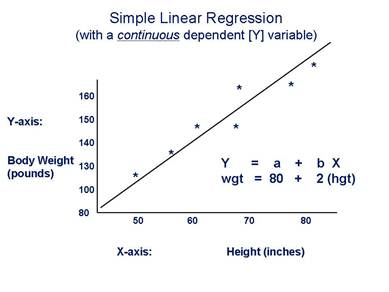
\includegraphics[center]{simpleLinearRegression}
	\caption[Confusion Matrix]
	{Simple Linear Regression}
	\label{fig:simpleLinearRegression}
\end{figure}

We can see from above the $y$ in this example is weight (wgt) and $b_0 + b_1x$ is $80 + 2*Height(hgt)$. This is a very basic example but demonstrates how this can be leveraged for more complex feature sets. Predicting arrears is a dichotomous problem meaning the outcome of the experiment can only have two possible values. 

\subsection{Logistic Regression} \label{LogReg}
\textit{Logistic Regression} \cite[See:][]{hosmer_applied_2000} within the credit scoring industry is one of the most used algorithms \citep{hand_evaluating_2010}. As seen above in Fig. \ref{fig:simpleLinearRegression} a simple regression model outputs a continuous response, in that example body weight. Credit scoring or predicting arrears is a problem where there can only be two possibly values default or not-default, to simplify this we will reduce this to a binary problem where the outcome will be 1 or 0 \citep{zou_modified_2004}. To transform the output of a regression model from $[-\infty, +\infty]$ to a probability between 0 and 1 a logistic transformation is applied. The logistic function can be used to take any value between $+\infty$ and $-\infty$ and output a value between $0$ and $1$. Fig. \ref{fig:logistic_function} below illustrates what a logistic function looks like.


\begin{figure}[H]
	\includegraphics[width=0.6\textwidth, center]{logistic_function}
	\caption[Standard Logistic Regression]
	{Standard Logistic Regression}
	\label{fig:logistic_function}
\end{figure}

The logistic function is defined in Equation \ref{eq:logitReg} as the following: 

\begin{equation} \label{eq:logitReg}
\text{Logistic Model}  =  p  =  \frac{1}{1 + e^{-(b_0 + b_1x)}}
\end{equation}

As discussed already linear regression is an unsuitable classifier for making dichotomous predictions as linear regression produces predictions for a range beyond 0 to 1. Logistic regression also produces a curved line that is bounded by values between 0 and 1. Fig. \ref{fig:LogRegVsLineReg}

\begin{figure}[H]
	\includegraphics[width=0.6\textwidth, center]{LogRegVsLineReg}
	\caption{Comparison between Linear and Logistic Regression Models}
	\label{fig:LogRegVsLineReg}
\end{figure}

in \ref{fig:LogRegVsLineReg} the constant, $b_0$ dictates the position of the curve which can be moved left and right depending on its value, $b_1$ will be the slope of the curve. 

The logistic regression model can be extended to include any number of interval and nominal variables which is illustrated in Equation \ref{eq:logitRegExtended}

\begin{equation} \label{eq:logitRegExtended}
p  =  \frac{1}{1 + e^{-(b_0 + b_1x_1 + b_2x_2 +\cdot\cdot\cdot+ b_px_p )}}
\end{equation}

Logistic Regression can also be used in cases where there are more than two outcome groups. For example it could be used in predicting what stage a customer is in the customer lifecycle e.g. Awareness, Interest/Consideration, Evaluation/Purchase, this is referred to \textit{multinomial logistic regression}


One of the main major attractions of logistic regressions it allows you to use discrete, continuous features or a combination of both \citep{lee_application_2005}.

\subsection{K-Nearest Neighbours} \label{kNN}
The \textit{k-nearest neighbour} or {k-NN} for short, is an algorithm that classifies observations based on the how its nearest neighbours are classified. It can be known as the nearest neighbour but in the majority of cases it is useful to use more than one neighbour \citep{henley_k-nearest-neighbour_1996}. The intuition behind this algorithm is that instances which are close by each other will more likely be classified the same way \citep{cover_nearest_1967}. We can see in Fig. \ref{fig:KNN_Example}\\ %added space for small gap in picture 


\begin{figure}[H]
	\includegraphics[width=0.6\textwidth, center]{KNN_Example}
	\caption{Example k-NN, contrasting results for \textit{k}=3 and \textit{k}=5 }
	\label{fig:KNN_Example}
\end{figure}

that results of the algorithm can vary with the choice of \textit{k}. It should also be noted that when applying this algorithm to binary experiment it is good practice to only choose odd values of \textit{k}, this will eliminate the risk of ties from the decision process \citep{keller_fuzzy_1985} 

While adopting the k-NN algorithm you can choose which method and validate what the best distance measure to decide what are your nearest neighbours. There are some common distance measures for continuous features only, Equation \ref{eq:Minkowski} is the \textit{minkowski distance} is one of the most common, where \textit{p=1} this becomes the Equation \ref{eq:Manhatten} the \textit{manhatten distance} and where \textit{p=2} this becomes the Equation \ref{eq:Euclidean} the \textit{euclidean distance}

\begin{equation} \label{eq:Minkowski}
\text{Minkowski Distance}   = \Big(\sum_{i=1}^k (\abs{x_i-y_i})^p\Big)^\frac{1}{p}
\end{equation}

\begin{equation} \label{eq:Manhatten}
\text{Manhatten Distance}   = \sum_{i=1}^k \abs{x_i-y_i}
\end{equation}

\begin{equation} \label{eq:Euclidean}
\text{Euclidean Distance}   = \sqrt{\sum_{i=1}^k (x_i-y_i)^2}
\end{equation}

The results from k-NN will vary depending on your choice of distance measurement, but there more distance metrics for continuous features such as \textit{Correlation Similarity}, \textit{Cosine Similarity} \citep{sarwar_item-based_2001}

Analysis can be completed to evaluate what the optimal value for \textit{k} is based on inspecting the results and creating benchmarks. Anecdotally the larger the value of \textit{k} the more precise the algorithm can be but as with most things in machine learning there are no guarantees. You can leverage methods such as cross validation discussed in Section \ref{subsec:k_fold} and utilised in Chapter \ref{Chapter4} to evaluate what the good choice of \textit{k} would be.

\subsection{Decision Trees} \label{decTrees}
The \textit{decision tree} algorithm classifies observations into classes in the form of tree like structure, hence the name. The algorithm seeks to partition the dataset into smaller subsets, using the relationship between the feature set and target variable to do so. Fig. \ref{fig:decisionTree}

\begin{figure}[H]
	\includegraphics[width=1\textwidth, center]{decisionTree}
	\caption{Simple Decision Tree for Yes, No Prediction \\ \cite[Source:][]{quinlan_induction_1986}}
	\label{fig:decisionTree}
\end{figure}

The output of the algorithm splits the data into smaller subsets of data, which output is a tree with root, internal and leaf nodes. As can be seen in Fig. \ref{fig:decisionTreeExplained}, the root node in this example \textit{Outlook} is the first node in the tree which means it is the most predictive feature. 

\begin{figure}[H]
	\includegraphics[width=.6\textwidth, center]{decisionTreeExplained}
	\caption{Decision Tree with Nodes and Leafs labelled}
	\label{fig:decisionTreeExplained}
\end{figure}

The \textit{root node} will have have two or more branches in this case three \textit{Rainy, Overcast} and \textit{Sunny}. Below these branches you have \textit{internal or split node} \textit{Windy} or \textit{Humidity} which output more branches. The bottom nodes of each decision or branch is the prediction or classification, this is called the \textit{leaf node}. In this example the leaf node decision will be whether or not it will rain represented by Yes/No in Fig. \ref{fig:decisionTreeExplained}

The algorithm that builds decision trees is called the \textit{iterative dichotomiser 3} more commonly known as ID3 by \cite{quinlan_induction_1986}. The algorithm applies a top down approach to choosing its root and internal nodes. The algorithm only evaluates one step ahead from where it is in the decision process at any time and does not allow for any backtracking. This decision making process is known as a greedy approach as it just makes the optimal solution at that stage of the process. Thus because of these limitations the optimal solution is not guaranteed taking this approach \citep{friedman_lazy_1996}.

The ID3 algorithm works by calculating the \textit{entropy} and \textit{information gain} at each step or decision node, where you use the feature with the smallest entropy or feature that maximises information gain.

Entropy $H(S)$ seen in Equation \ref{eq:entropy} measures how much uncertainty there is in the data \citep{shannon_mathematical_2001}

\begin{equation} \label{eq:entropy}
H(S) = - \sum_{x \in X} p(x) \log_{2} p(x)
\end{equation}
Where:
\begin{itemize}[label=]
	\item $S$: The current dataset entropy is being calculated for, this will change each time entropy is being calculated
	\item $X$: The set of classes in $S$
	\item $p(x)$: Proportion of observation in class $x$ compared to total number in set $S$
\end{itemize}
If $H(S) = 0$ then the observations in $S$ are all of the same class. Entropy is calculated for each feature, the feature with the smallest entropy is used to split at that step.

Information gain is used to measure the decrease in entropy after the dataset is split on a feature. The equation for the information is 

\begin{equation} \label{eq:infoGain}
IG = H(S) -  H(T)
\end{equation}
Where:
\begin{itemize}[label=]
	\item $H(S)$ is the the entropy of S
	\item $H(T)$ is the entropy of subset T based on splitting data on some feature
\end{itemize}

Information gain is calculated and the feature with the highest gain is chosen to split the dataset. The algorithm then runs recursively until all the data is classified and predictions have been made. 

Multiple decision trees may output the same results. This can be seen in Fig. \ref{fig:simpleComplex} where two different decision trees classify the dataset correctly. \cite{quinlan_induction_1986} suggests that that in scenarios like this the simpler decision tree would be chosen Fig. \ref{fig:simple}

\begin{figure}[H]
	\centering
	\begin{subfigure}[b]{0.45\textwidth}
		\captionsetup{font=scriptsize}
		\includegraphics[width=\textwidth, height=5cm]{decisionTreeSimple}
		\caption{Simple Decision Tree}\label{fig:decisionTreeSimple}
		\label{fig:simple}
	\end{subfigure} ~\quad
	\begin{subfigure}[b]{0.45\textwidth}
		\captionsetup{font=scriptsize}
		\includegraphics[width=\textwidth,height=5cm]{decisionTreeComplex}
		\caption{Complex Decision Tree}\label{fig:decisionTreeComplex}
		\label{fig:complex}
	\end{subfigure}
	\caption{Simple and Complex Decision Tree Comparison\\\cite[Source:][]{quinlan_induction_1986}}
	\label{fig:simpleComplex}
\end{figure}

This is done because the simpler the rules of the tree the more likely the tree is to generalise well on unseen data. In other words if the tree is too complex it is more than likely over-fitting the training dataset. There is also a computational cost to classifying complex trees. 

There are also other issues to be aware of when building a classifier using a decision tree. Information gain can be biased to features that have a large number of values. These features will result in a root node that produces a very broad or wide tree that classifies the training data well or perfectly but performs very poorly in unseen cases. One scenario where this could happen would be if you used the unique identifier of each record in as a training input, this model would perform very well in training but would not perform well on unseen data. There are methods to mitigate the the risk of over-fitting against these features \textit{gain ratio}, \textit{symmetric uncertainty} and the \textit{gini index}. \cite{quinlan_induction_1986} noted that using these methods for node decision often found favourable results compared with information gain. It should be noted also that these metrics can be using in the feature selection process where not related to building decision trees

\subsection{Ensemble models \& Boosting} \label{boosting}
\begin{comment}

In 1907, statistician Sir Francis Galton attended a fair in which there was a competition to judge the weight of an Ox. Upon reviewing the 787 predictions made by the competing public, he observed that while there was a 
\end{comment}

\subsection{Neural Networks} \label{neuralNets}
Neural Networks in broad terms are a class of model that attempt to learn patterns in data by simulating the activity in a human brain.


\subsection{Support Vector Machines} \label{SVM}
Support Vector Machines (SVM) were developed from Statistical Learning Theory 

%----------------------------------------------------------------------------------------
%	SECTION 8
%----------------------------------------------------------------------------------------
\section{Class Imbalance Problem}
One of the biggest assumptions that needs to be understood when using classification algorithms is that most assume there is a balanced distribution of the target class \citep{japkowicz_class_2000}. Target class imbalance is described by  \citep{chawla_smote:_2002} where the number of number of records in each class are not relatively equal. In a balanced dataset ratio between the a binary target class would be close to 50/50. The issue with this imbalance arises where algorithms assume there is a balance between the classes, and they attempt to maximise the accuracy by predicting the most common class \citep{drummond_severe_2005}. The algorithms attempt to minimise the classification errors, but do not accounts for the incorrectly classifying cases \citep{seiffert_improving_2009}. While these classification overall might be very accurate they are not very useful in real world problems, this is because in the majority of cases the algorithm will focus on the majority class, because of how heavily it is weighted in the training dataset ignoring the minority class. This is major problem because in the majority of cases you will trying to predict the minority class, in this thesis customers going into default is the minority e.g. there are more customers that do not default at the end of the outcome window than customers that do defaulters.

The study of class imbalance has started to receive more and more attention in relation to data mining and machine learning in recent times. \cite{weiss_mining_2004} discusses what the role and issue that rare class instances can play in data mining. \cite{weiss_mining_2004} makes the distinction that there are two types of class imbalance which depend on the type of rarity in the data, these are called \textit{absolute rarity} and \textit{relative rarity} which are discussed next.

The major issue with rarity is there is a simply a lack of data in real world problems. Absolute rarity occurs when the number of instances related to the rare class is very small in an absolute sense. Lack of data means it is difficult to identify what leads to a rare class. Fig. \ref{fig:absoluteRarity} illustrates how absolute rarity can become an issue.

\begin{figure}[H]
	\includegraphics[width=0.6\textwidth,center]{absoluteRarity}
	\caption{
				Impact of Absolute Rarity in Data Mining \\ \cite[Source:][]{weiss_mining_2004}
			}
	\label{fig:absoluteRarity}
\end{figure}

It can be seen on the left side of Fig. \ref{fig:absoluteRarity} that there is only one rare/positive example, compared to the right where there is more data this more rare cases. It can be observed that the decision boundary on the right side for when there is more data is much more accurate than on the left side when there is just one observed rare class. This is a simple illustration that having more data should allow you to make better predictions. Relative rarity is where classes are not rare in an absolute sense but are rare relative to other objects. A supermarket example can illustrate this better, imagine you want to identify the relationship between two items, but these items are rarely purchased as whole, so even if they happen to be purchased together the relationship may be difficult to identify.

As mentioned previously, very often in the real world problems imbalance exists in the dataset, thus there has been researched completed that have identified methods of mitigating against this risk. \citep{chawla_editorial:_2004} proposes solutions fine tuning the algorithm and manipulating the data. 

\subsection{Manipulating the data}

A method of manipulating the data is to resample to data with the aim of balancing the distribution of the target class. Solutions proposed,

\begin{itemize}
	\item Random undersampling the majority class
	\item Random oversampling the minority Class
	\item Synthetic of the minority Class 
\end{itemize}

A very common method used is to randomly oversample the minority class in your training set, one of the biggest issues with this is that you are increasing your chances of over-fitting the algorithm the training model as it been training on multiple copies of the same data which are not adding any new information. However over-fitting can be issue with this approach as the algorithm becomes biased and skewed on the training data, thus ends up performing poorly on the validation and test data \cite[see][]{hawkins_problem_2004}

Random undersampling of the minority class is where random samples of the training dataset that are part of the majority class are removed. This means number of minority classes remains unchanged but the majority class is reduced, thus the overall class balance becomes more even. The issue that arises from undersampling is that there is possibility that you removes the important information from the training dataset that is used for predicting that class. It should be noted \cite{kennedy_credit_2013}, that undersampling the majority class is not a useful solution for the issue of absolute rarity.

Synthetic sampling  is alternative method to randomly oversampling the minority class. New data items are added to the training set but unlike oversampling which adds duplicate records the records added are dummy or made up in a way to look similar and taking characteristics of the already existing records, thus they are not duplicates but synthetic. One method for creating synthetic data was proposed by \citep{chawla_smote:_2002} where data was generated by creating data items using K-NN where the item would sit between minority classes. 

\begin{figure}[H]
	\centering
	\begin{subfigure}[b]{0.32\textwidth}
		\captionsetup{font=scriptsize}
		\includegraphics[width=\textwidth]{SMOTE_Before}\caption{}
		\label{fig:SMOTE_Before}
	\end{subfigure}  ~\quad
	\begin{subfigure}[b]{0.32\textwidth}
		\captionsetup{font=scriptsize}
		\includegraphics[width=\textwidth]{SMOTE_After}
		\caption{}
		\label{fig:SMOTE_After}
	\end{subfigure}
\caption{Fig. \ref{fig:SMOTE_Before}: Example of the K-NN for $x_i$ using $k = 6$. \ref{fig:SMOTE_After}: Data created using SMOTE based on the euclidean distance.\\
	\cite[Source:][]{he_learning_2009}}
\label{fig:smoteExample}
\end{figure}

Above in Fig. \ref{fig:smoteExample} it is illustrated how synthetic data using the SMOTE methodology can be generated. For the purposes of this thesis this will not be discussed further.

\subsection{Fine tuning the algorithm}
There are ways to also cater for the target class imbalance of the dataset by fine tuning the algorithm. One method which is illustrated in Chapter \ref{Chapter4} of this thesis is to adjust the cut-off or threshold parameter value for the model, \cite{provost_machine_2000} warns that it would \textit{``critical mistake"}. In Section \ref{modelPerformMeasure} model performance measures, it is  worth noting that \cite{chawla_editorial:_2004} suggests using evaluation measures such as accuracy which rely on a specific threshold could lead to misleading results when the target class is imbalanced, they instead recommend using ROC and AUC to get a more accurate predictions, this similar to industry standards in terms of handling the imbalance.

This section has detailed some of the concern that imbalance can cause when building predictive models, we have outlined some the solutions and methods to mitigate this by manipulating the data and fine tuning the classification algorithm.

%----------------------------------------------------------------------------------------
%	SECTION 8
%----------------------------------------------------------------------------------------
\section{Model Validation Methods}
In machine learning historic data is used to build a model to make future predictions based on past information. Classification algorithms like the ones already discussed in this section need to validated and tested. This section details some methods and approaches to tackling this problem so the predictions from the model are useful which has been discussed extensively in \citep{refaeilzadeh_cross-validation_2009}

\subsubsection{Resubstitution Validation}
The \textit{resubstitution validation} method the model is trained using the full dataset available, and afterwards tested using the same dataset. The results of this test will most likely be positive, but there os a danger that the model will perform poorly on unseen data because it because it is over-biased and over-fits the training data

\subsubsection{Holdout Validation}
The \textit{holdout validation} method is used to avoid the over-fitting issue discussed in the resubstitution method. The idea is to split the data into partitions, one for training and one for testing. The algorithm is only trained on the test data, this allows for the model to generalise much better on unseen data, overall producing a much better prediction model. This method has an issue however where one, not all the data is used for training, and two the results can be dependent on the how and what data are used for training and testing. Examples where this could become an issue is important information in the data for training is lost in the test partition, or the instances chosen for test may be too easy or too difficult to classify, this may cause your results to be skewed and making your predictions bias to that testing partition.

\begin{figure}[H]
	\includegraphics[width=0.6\textwidth,center]{holdout}
	\caption{Example of Holdout Validation Data Split}
	\label{fig:holdout}
\end{figure}

Fig. \ref{fig:holdout} illustrates how the complete dataset is partitioned into a training and test sets. To address the biasses is Holdout you could re-run multiple tests and average the results, or more commonly you could look at using \textit{k-fold cross-validation} discussed in the next subsection.

\subsubsection{K-Fold Cross Validation}\label{subsec:k_fold}
The \textit{k-fold cross validation} can be used to deal with the bias issues discussed above. The first step of this method is to split the data into $k$ equally sized partitions called folds. A model is then trained using $k$ iterations, where for each iteration a different fold of data is used for testing and training the model. This can be illustrated well below in Fig. \ref{fig:5-fold-cv} where there are 5-folds, and for each iteration you can see different fold is being used for testing.  

\begin{figure}[H]
	\includegraphics[width=0.7\textwidth,center]{5-fold-cv}
	\caption{5-Fold Cross Validation}
	\label{fig:5-fold-cv}
\end{figure}

It is important and usually common practice that each fold is representative of the the whole dataset, for each example that the target class ratio split is the same for each fold as for the entire dataset. 

\subsubsection{Leave-One-Out Cross-Validation}
The \textit{leave-one-out cross-validation} (LOOCV) method is a specialised version of $k$-fold cross-validation, where $k$ is equal to the number of observations in the dataset. In layman's term this means all the data bar one observation is utilized training the model, and testing is done on one observation. This is completed for each observation in the dataset. Although it is worth noting that accuracy estimate gathered using this method produces unbiased results, it also high variance which can lead to misleading results \citep{refaeilzadeh_cross-validation_2009}.
 

\subsubsection{Repeated K-Fold Cross Validation}
The \textit{repeated k-fold cross validation} method is another specialised version of $k$-fold cross-validation. In an attempt to improve the performance of the model using this method $k$-fold cross-validation is rerun multiples times. Each time it is rerun the data is shuffled so data will appear in different folds for each repeat run. 

\subsubsection{Summary}

Holdout and cross validation methods are both used extensively for evaluating how measuring the performance of the models. In the majority of cases if there is a large enough dataset you might choose to just use holdout method, but in some situations of you may want to use cross validation.

There are considerations that need to be thought about before using either, hold-out is simple can be implemented easily and quickly and can be rerun multiple times to get a more unbiased result. K-fold is again theoretically simple but may not be a simple to implement as the code may be tedious and time consuming where the gains may not be worth the investment in industry. 

\citep{kohavi_study_1995} and \citep{salzberg_comparing_1997} both performed research on approaches to choosing the correct validation method. \cite{kohavi_study_1995} analysed many cross validation methods, regular, leave-one-out, stratified. They came to the conclusion that 10-fold cross-validation produced the most accurate and unbiased results. \cite{salzberg_comparing_1997} also studies the issues of comparing model performance and proposes a solution that combines k-fold cross validation combined appropriate hypothesis tests opposed to evaluating the average accuracy.   

%----------------------------------------------------------------------------------------
%	SECTION 9
%----------------------------------------------------------------------------------------
\section{Model Performance Measures}\label{modelPerformMeasure}

This section details some of the metrics that can be used to assess the accuracy of a classifier. The result of the classification algorithm maps the modelled data into a category, in this thesis it a binary classifier that is output: 1 is output for identifying customers who will default (bad) or 0 is output for customers who will be not-default (good). The majority of classification algorithms will produce a ranked numeric value which can be converted to a binary representation by some threshold or cut-off decision driven from  the business objective that is trying to be optimised. This section will begin with a confusion matrix, details how this is leveraged to build other performance measures and details how charts and metrics can be leveraged together to decide on the performance measure to maximise the intended objective.

\url{http://www.saedsayad.com/model_evaluation_c.htm}

\subsubsection{Confusion Matrix}

The results that made by the classification algorithm can be represented by a contingency table known as a confusion matrix. In this thesis the classification algorithm will output a binary classification, so the confusion matrix will be made from a $2 \times 2$ matrix that has two classes, known as the \textit{positive} and \textit{negative} class. For this thesis, the positive class will be the customers that default and negative class will be the customers that do not default. It will illustrate what proportion of correct and incorrect predictions were made with respect to the target.The confusion matrix can be broken down into the following categories for this thesis:

\begin{itemize}
	\item \textit{true positive} (TP), cases that are predicted to default, and are {\color{green}{correctly}} classified as \textit{positive}
	\item \textit{false positive} (FP), cases that are predicted to default, and are {\color{red}{incorrectly}} classified as \textit{positive}, also known as \textit{Type I error}.
	\item \textit{false negative} (FN), cases that are predicted to not-default, and are {\color{red}{incorrectly}} classified as \textit{negative}, also known as \textit{Type II error}.
	\item  \textit{true negative} (TN), cases that are predicted to not default, and are {\color{green}{correctly}} classified \textit{negative}
	
\end{itemize}

Fig \ref{fig:ConfusionMatrix} illustrates how information from a confusion matrix can be presented and read.

\begin{figure}[H]
	\includegraphics[width=0.8\textwidth,center]{Confusion_Matrix}
	\caption[Confusion Matrix]
	{Confusion Matrix}
	\label{fig:ConfusionMatrix}
\end{figure}

Using the numbers outputted from the confusion matrix, model evaluation measures can calculated and evaluated for the required objective, measures such as \textit{accuracy} (Equation \ref{eq:Accuracy}) which measures proportion of the number of predictions that were correct, the \textit{misclassification rate} (Equation \ref{eq:Misclassification Rate}) what proportion of predictions were wrong, the \textit{sensitivity} (Equation \ref{eq:Sensitivity}), otherwise known as \textit{recall} or the \textit{true positive rate} (TPR), measures the proportion of the positive instances that are correctly identified i.e. proportion default cases that have been predicted correctly. \textit{Specificity} (Equation \ref{eq:Specificity}) measures the proportion of negative cases that are predicted correctly i.e. proportion of non-default cases that have been predicted correctly, \textit{precision} (Equation \ref{eq:precision}) measures when the classifier predict positive outcomes what proportion are correct, \textit{negative predictive value} (NPV) (Equation \ref{eq:npv}) measures the proportion of negative predictions that were correct i.e. if the classifier predicted the outcome would be non-default what proportion were correct. One measure that can be very useful when the where there is class imbalance is \textit{balance accuracy} (Equation \ref{eq:Balanaced Accuracy}), \citep{brodersen_balanced_2010} discusses how using this negates the impact of bias or skewness from the more frequent class

\begin{equation} \label{eq:Sensitivity}
\text{Sensitivity} = \text{Recall} = \frac{TP}{TP + FN}
\end{equation}

\begin{equation} \label{eq:Specificity}
\text{Specificity} = \frac{TN}{FP + TN}
\end{equation}

\begin{equation} \label{eq:precision}
\text{Precision} = \frac{TP}{TP + FP}
\end{equation}

\begin{equation} \label{eq:npv}
\text{Negative Predictive Value} = \frac{TN}{TN + FN}
\end{equation}

\begin{equation} \label{eq:Accuracy}
\text{Accuracy} = \frac{TP + TN}{TP + FP + FN + TN}
\end{equation}

\begin{equation} \label{eq:Balanaced Accuracy}
\text{Average Accuracy} = \text{Balanaced Accuracy} = \frac{Sensitivity + Specificity}{2}
\end{equation}

\begin{equation} \label{eq:Misclassification Rate}
\text{Misclassification Rate} =  \frac{FP + FN}{TP + FP + FN + TN} = 1 - \text{Accuracy}
\end{equation}

\begin{figure}[H]
	\includegraphics[width=0.8\textwidth,center]{Confusion_Matrix_Example}
	\caption[Confusion Matrix Example]
	{Confusion Matrix Example}
	\label{fig:ConfusionMatrixExample}
\end{figure}

Fig. \ref{fig:ConfusionMatrixExample} illustrates how the TP, FP, FN, TN can be used to create performance metrics for classification algorithm. As discussed already confusion matrix based performance measures are built on the threshold that is selected for converting the predicted numeric score into a binary outcome. Anecdotally you might believe that the cut-off or threshold of 0.50 is acceptable but this rule may not always especially if there is an imbalance between the positive and negative class in the dataset. The cut-off should should ideally be based on you business objective where you look to minimise, maximise and analyse the trade off as you alter the cut-off. 

The confusion matrix is not the only way to evaluate the performance of the classification algorithm and is not always advocated in the literature or by industry. In studies completed by \citep{lessmann_benchmarking_2008} choose not to select a classification cut-off arguing that studies comparing the same dataset and classifier could come to the different conclusions.

As mentioned in this section the confusion matrix measures the performance of classifier at a specific threshold, this can be leveraged to create graphical representations of the overall fitness of the model at any threshold. One such method that will be discussed in the next section is the \textit{receiver operating characteristic} (ROC). 


Confusion Matrix is used to evaluating a model where you have divided the output into distinct or discrete categories. A confusion matrix can be reconstructed for any point on the ROC curve. ROC is also is directly related to two other performance methods \textit{area under the curve} and \textit{gini} which will also be discussed.  

\subsubsection{ROC Chart, AUC and Gini Coefficient}
%\url{https://staesthetic.wordpress.com/2014/04/14/gini-roc-auc-and-accuracy/}
The ROC chart is used to evaluate and illustrate how well the evaluate the model fit, this can be a quick test to see if the model generalises well from the test data, to validation and test data. Fig. \ref{fig:ROC} illustrates on the \textit{x-axis} the false positive rate, and on the \textit{y-axis} the true positive rate is represented. As mentioned previously the points on the ROC chart are generated from confusion matrix built from many cut-off or threshold value between $\theta \in [0,1]$. Fig. \ref{fig:ROC} conceptually illustrates how the ROC chart is generated for varying thresholds. 

\begin{figure}[H]
	\includegraphics[width=0.8\textwidth,center]{ROC}
	\caption[ROC]
	{ROC Chart Example with thresholds 0.65 \& 0.50}
	\label{fig:ROC}
\end{figure}

Fig. \ref{fig:ROC} also illustrate how point (0,1) represents \textit{perfect classification}, that is the classifier correctly predicts all outcomes. 

The ROC chart is basically a combination of confusion matrices over many cut-off values of a classifier. As you can see above finite number of observations in the dataset dictates the number of thresholds that can be used to generate a ROC chart.

To compare ROC chart results of different classifiers the \textit{area under the ROC curve} (AUC) \citep{bradley_use_1997} \& \citep{hanley_meaning_1982}. In Fig. \ref{fig:ROC} the area under the blue ROC line represents the AUC, which is intuitively the area under the curve. In the case of perfect classification this value will be 1, for a random classifier the AUC would be 0.5. 

It is worth noting that AUC does not give total probability of the classifier, and also its usefulness when combined with the ROC to evaluate your classifier across training, validation and test datasets. For example if the ROC curve shifts significantly or is not similar from training to validation/test it suggests that there is possible over-fitting and the model does not generalise well. Also it is worth looking out for a drastic change in the AUC from training to validation/test another sign the classifier does not generalise well may not be useful for predictions. Because of this it is a very strong measure for classifier selection, ROC don't tend to cross over, therefore when comparing two classifiers the one which AUC is higher will be the better classifier independent of the threshold or cut-off.

It is illustrated in Fig. \ref{fig:matric_compare} how the performance measures for confusion matrices vary for different thresholds, but again to keep in mind that it there be just one measure for the AUC of the this ROC Chart.   

\begin{figure}[H]
	\centering
	\begin{subfigure}[b]{0.45\textwidth}
		\captionsetup{font=scriptsize}
		\includegraphics[width=\textwidth]{Confusion_Matrix_threshold_065}
		\caption{Threshold $=.65$}\label{fig:Threshold65}
	\end{subfigure} ~\quad
	\begin{subfigure}[b]{0.45\textwidth}
		\captionsetup{font=scriptsize}
		\includegraphics[width=\textwidth,height=2.025cm]{Confusion_Matrix_threshold_050}
		\caption{Threshold $=.50$}\label{fig:Threshold50}
	\end{subfigure}
	\caption{Confusion Matrix: Multiple Threshold Comparison}
	\label{fig:matric_compare}
\end{figure}

A metric that is commonly used for in \subjectname, industry credit scoring is the \textit{gini coefficient} this is discussed in \citep{hand_good_2005}, this is equates to twice the area in between the diagonal of a random classifier and the ROC curve. The equation for this can be seen below in Equation \ref{eq:gini}

\begin{equation} \label{eq:gini}
\text{Gini} = 2*\text{AUC} - 1
\end{equation}

Just like using a threshold there are limitations to using the AUC and Gini to measure classifier performance, although extremely useful for analysing the performance of wide range of thresholds but not as useful when trying to maximise the performance over a narrow range of thresholds. It cannot tell us the optimal threshold for classifier for  other statistical needs.

One statistic that is commonly used in credit scoring in \subjectname\, industry and in the literature is the \textit{kolmogorov-smirnov} (KS) statistic, this will be discussed in the next subsection.
	

\subsubsection{K-S Chart}\label{subsub:ks}
%\url{http://www.saedsayad.com/model_evaluation_c.htm}
The KS chart and more specifically the KS statistic is one value between 0 and 1. It can be used by measuring the performance of the classifier, by measuring the maximum distance between the cumulative positive and negative distributions of the predicted positive and negative class \citep{seliya_study_2009}. In other words K-S is a measure that illustrates the maximum seperation between the positive and negative distributions, this can illustrated more clearly in Fig. \ref{fig:ks}.

Fig. \ref{fig:ks} how the KS statistic and chart is generated, probabilities from the classifier are ordered, grouped and aggregated, but importantly they are separated by the positive and negative class, creating a distribution for each. These two distributions are then plotted separately, you can see in Fig. \ref{fig:ks} that the KS statistic is 47.4\%. This is calculated by taking maximum difference between the two distributions at each group. At group 400-500, if you were to classify all the score are positive below or in this group you would be identifying 81.7\% of the positive instance and only 34.3\% of the negative class, if this was a balanced dataset this could be a very valuable result and measure. 

\begin{figure}[H]
	\includegraphics[width=0.8\textwidth,center]{ks}
	\caption[Kolmogorov-Smirnov chart ]
	{Kolmogorov-Smirnov Table \& Chart }
	\label{fig:ks}
\end{figure}

There are extreme cases of the KS statistic that are worth noting, on is where the KS statistic is equal to 100, this means the scores for each distribution (positive/negative) are but into two separate groups, where one group would just have positive cases and the other just negative case. Alternatively if the model is not very useful and cannot tell the positives from the negatives, it will be like the model is selecting cases randomly and will return a KS statistic of 0.

We will see Chapter \ref{Chapter4} how this statistic can be utilised and leveraged to create a useful threshold value. 

\subsubsection{Gain \& Lift}
The \textit{gain} \& \textit{lift} measure the performance of the classifier. One example where these measure as charts are extremely useful is when communicating in industry with management, they are easy to explain and intuitive where the business can derive and understand value immediately. Fig. \ref{fig:GainLiftWorkflowCharts} below illustrates how the gain and lift charts are generated. 

\begin{figure}[H]
	\centering
	\begin{subfigure}[b]{0.90\textwidth}
		\captionsetup{font=scriptsize}
		\includegraphics[width=\textwidth,height=4cm]{gains_ratio_process}\caption{Process}\label{fig:gains_ratio_process}
	\end{subfigure} 
	\medskip
	\newline
	\begin{subfigure}[b]{0.45\textwidth}
		\captionsetup{font=scriptsize}
		\includegraphics[width=\textwidth]{gains}
		\caption{Gain Chart}\label{fig:gains}
	\end{subfigure} ~\quad
	\begin{subfigure}[b]{0.45\textwidth}
		\captionsetup{font=scriptsize}
		\includegraphics[width=\textwidth]{lift}
		\caption{Lift Chart}\label{fig:lift}
	\end{subfigure}
	\caption{Gain \& Lift Work-flow \& Charts}
	\label{fig:GainLiftWorkflowCharts}
\end{figure}

The charts above illustrate how much likely it is we receive positive responses using the classifier compared to use a random model. The population in the dataset are broken into deciles, which can be seen in \ref{fig:gains} \& \ref{fig:lift}. An example of how they can be used is if we were to evaluate the first 10\% of the population identified by the classifier it would outperform a random selection of customers that would turn out to positive by 3.6.

Essentially these charts are visual aids which can be leveraged for evaluating the performance of the classifier. 

%----------------------------------------------------------------------------------------
%	SECTION 5
%----------------------------------------------------------------------------------------
\section{Conclusion}\label{sotaConc}
This chapter has summarised the relevant literature available for two-class classification and web data analysis, with discussion of predicting future behaviour based on sequential click patterns. Various models have been discussed including K-Nearest Neighbours, Association Rules, Decision Trees, SVM, Neural Networks, Regression Models and ensemble models

%----------------------------------------------------------------------------------------
%	SECTION 6
%----------------------------------------------------------------------------------------
 
% Chapter Template

\chapter{Data} % Main chapter title

\label{Chapter3} % Change X to a consecutive number; for referencing this chapter elsewhere, use \ref{ChapterX}

\lhead{Chapter 3. \emph{Data}} % Change X to a consecutive number; this is for the header on each page - perhaps a shortened title

%----------------------------------------------------------------------------------------
%	SECTION 1
%----------------------------------------------------------------------------------------
\section{Introduction}
This chapter presents the data that will be used for the experiments to be carried out in this research and will be split into two main sections. 

The first section will outline where the customers for the experiment have been gathered from, and under what criteria they have been selected. As part of the experiment a baseline predictive model will be built, this will be done using features that were used in historic industry credit scorecard models in \subjectname. Performance measure measure will also selected evaluated also using this base line analysis later seen in Chapter \ref{Chapter4}.

The second section will outline what macro-economic features will be built as part of the experiment in this research. The aim of this research is to investigate the predictive power of macro-economic features by geographic regions such as electoral divisions and local authority in Ireland. To do this the addresses that are stored in \subjectname's databases are queried against an search engine and string metric algorithm application built for this research map addresses to \textit{global positioning system} (GPS) coordinates. The macro-economic features will be sourced and created from internal data sources in \subjectname\ and externally from open data sources. It will also explain how these features have been created, what transformations or data wrangling had to be done so the features fit/map into an analytical base table (ABT) discussed in Section \ref{sec:datasetConstruction} that is a requirement for predictive modelling. Care was also taken throughout this experiment to ensure that anachronistic variables were not included in any of the  built as part of this research e.g. Features that contains information about the outcome after the time the observation point. 

\section{Experiment Set-up}
This section will detail data is in scope for prediction in this research. In Fig. \ref{fig:experiment_setup1} below SME customers are selected at the \textit{observation point}, June 2014. These customers are not in default at this point in time. Information prior to the observation point will be used for modelling to predict if a customer is likely to go into default, this is known as the \textit{performance window}.

Data from each individual customers performance will be taken from data in the performance window time period, which will be combined with macro location-based data prior to the observation point also. This data will be aggregated and structured into features for an ABT. The aim will be that these features will be able to distinguish what customers are likely to default on there repayment in the next 12 months. 

\begin{figure}[H]
	\includegraphics[width=0.8\textwidth,center]{experiment_setup}
	\caption[Experiment Performance Window and Outcome Window]
	{Experiment Performance Window and Outcome Window}
	\label{fig:experiment_setup1}
\end{figure}

Previous, Section \ref{classLabelDef} described that there were two methods used to define if a customer was in default or not: (i) the \textit{worst status} label definition method; and (ii) the \textit{current status} label method approach. As mentioned previously, for the purpose of this experiment we will be using the industry standard worst status method, this means if the customers is in 90+ days arrears at any stage in the outcome window they will be labelled as a bad customer or as one that has defaulted on their financial obligation. 


\section{Customers for Credit Scoring and Existing Features}\label{sec:existFeatures}

The customer data used for prediction in these experiments was sourced from a financial institution \subjectname, which is one of the two main pillar banks in Ireland. It contains details of 27,082 SME customers who were active between June 2014 and June 2015. These 27,082 customers are a subset of SME customers on the \subjectname\ book as the experiment will only be completed on one of the loan systems in the financial institution. None of the 27,082 customers are in default at the observation point(June 2014). The baseline model for this experiment will be built from features from a historic scorecard in \subjectname.

As mentioned in Section \ref{sec:segment} it is very common in credit scoring to model the population into multiple groups. This is done so homogeneous customers are grouped and modelled together based on for example pattern, characteristic, demographic etc. This common practice in industry also, in \subjectname\ is one method of modelling the credit risk of customers by splitting the customers into two segments. The criteria for selecting which segment each customer is modelled in is if that customer has been in arrears previously or not. For for this research a customer will be modelled in the \textit{Previous Delinquency} segment, if the customer \textbf{has not been} performing well and been in arrears previously. If the customer \textbf{has been } performing well and not been in arrears previously they will be modelled in the \textit{No Previous Delinquency} segment. The historic scorecards that were used in \subjectname\ used different features to build a model for each segment population. This was done using empirical analysis of the data where it was observed that different features contributed to the prediction of each subset of the population with a few overlapping features in each subset. Due to sensitivity of the information in \subjectname, the feature set for these models could not be documented in this research paper.

As mentioned in Section \ref{sec:imBalance} class imbalance in datasets is a major real world problem when building a predictive model. As mentioned previous this happens when the target class is is not distributed evenly in the dataset. The dataset in this experiment suffers from this imbalance also, however because the data is partitioned into two segments the imbalance in \textit{previous delinquency} dataset improves significantly but gets worse in the \textit{no previous delinquency} dataset.

The characteristics of the two datasets that will be used to build the baseline benchmark can be illustrated in Table \ref{characteristicsDatasets} below.

\begin{table}[H]
	\centering\
	\resizebox{\textwidth}{!}
	{
		\begin{tabular}{l r r r r r r}
			\hline
			\textbf{Model} &  \textbf{\# Numeric} & \textbf{\# Nominal} & \textbf{\# Observations} & \textbf{\# Good} & \textbf{\# Bad} & \textbf{Good:Bad}\\
			\hline
			Previous Delinquency & 11 & 0 & 2,926 & 2,198  & 738 & 75:25 \\ 
			No Previous Delinquency & 9 & 0 & 24,156 & 23,505 & 651  & 97:03 \\ \hline
			\textbf{Total} &  &  & \textbf{27,082} & \textbf{25,703} & \textbf{1,389} & \textbf{95:05} \\ \hline
		\end{tabular}
	}
	\caption{Characteristics of datasets to be used in the exploratory evaluation for training a benchmark model and assessing the evaluation metrics to be used in the research \\
		 \# Numeric refers to the number of continuous features \\
		 \# Nominal refers to the number of categorical features
		}
	\label{characteristicsDatasets}
\end{table}

It can be seen above in Table \ref{characteristicsDatasets} that two datasets are not very similar. There are only 2,936 customers in the \textit{previous delinquency} dataset and 24,156 in the \textit{no previous delinquency} dataset. Perhaps the the biggest difference is class imbalance difference between the datasets. 25\% of customers in the \textit{previous delinquency} dataset are bad by the end of the outcome window but there is only 3\% of the \textit{no previous delinquency} dataset that are bad at the end of the outcome window. As discussed in Section \ref{sec:imBalance} this presents significant challenges when try to build a predictive model but also a very common challenge in real world applications. 


\section{Macro-Economic Areas for Experiment}
The experiment in this research is to investigate if macro-economic features by locations are useful for predicting if SME customers are likely to go into default. The two macro-economic regions that features will be based on are \textit{Electoral Division} (ED) and \textit{Local Authority} (LD). Below Fig. \ref{fig:Ireland_ED_LA_Example} maps out the electoral divisions and local authorities in the Republic of Ireland.

\begin{figure}[H]
	\begin{subfigure}[b]{0.5\textwidth}
		\captionsetup{font=scriptsize}
		\includegraphics[width=\textwidth,height = 10cm]{IrelandElectoralDivisions}
		\caption{Map of the Current 3,440 Electoral Divisions}\label{fig:IrelandElectoralDivisions}
	\end{subfigure} ~\quad
	\begin{subfigure}[b]{0.5\textwidth}
		\captionsetup{font=scriptsize}
		\includegraphics[width=\textwidth,height = 10cm]{IrelandLocalAuthorities}
		\caption{Map of the Current 34 Local Authorities}\label{fig:IrelandLocalAuthorities}
	\end{subfigure}
	\caption{Republic of Ireland's Electoral Divisions Local Authorities}
	\label{fig:Ireland_ED_LA_Example}
\end{figure}

There are 34 primary local authorities in the Republic of Ireland, including 29 county councils and 5 city councils. Organisations within each area are responsible for managing issues such as housing, planning, roads, water supply and sewerage, development incentives and controls, environmental protection, recreation facilities and amenities, agriculture, education, health and welfare \footnote{\url{http://www.iro.ie/local_authorities.html}}. There are 3,440 electoral divisions in the Republic of Ireland. Electoral divisions are formed by grouping town-lands together and are the smallest legally defined administrative areas in the state which small population statistics are published from in the Census \footnote{\url{http://census.cso.ie/censusasp/saps/boundaries/eds_bound.htm}}.


\section{Converting Addresses to GPS Coordinates}
To link macro-economic features by electoral division and local authorities to a SME customer there has to be a mechanism. In an ideal world this would be done through a data model where a customers address would be linked to the address reference database. This can be illustrated through the Entity-Relationship Model (ERD) in Fig. \ref{fig:MasterReferenceAddressDataArchitecture}.

\begin{figure}[H]
	\includegraphics[width=1\textwidth,center]{MasterReferenceAddressDataArchitecture}
	\caption{Optimal Entity Relationship Data Model for Mapping Customers, Addresses, Electoral Division and Local Authorities}
	\label{fig:MasterReferenceAddressDataArchitecture}
\end{figure}

Unfortunately this is not the case currently in \subjectname. Currently addresses are stored in free text fields across multiple systems. This can be illustrated in Fig. \ref{fig:AIB_Situtation} where you can see unstandardised and free text addresses are stored in the Customer table instead of an address reference table like in Fig. \ref{fig:MasterReferenceAddressDataArchitecture}.

\begin{figure}[H]
	\includegraphics[width=.7\textwidth,center]{AIB_Situtation}
	\caption{Current Entity Relationship Data Model for Mapping Customers, Addresses, Electoral Division and Local Authorities}
	\label{fig:AIB_Situtation}
\end{figure}

With the release of Ireland's new postcode system in July 2015 Eircode\footnote{\url{http://www.eircode.ie/}} \subjectname\ was looked to position itself strongly for its deployment and how it would integrate into \subjectname's current systems. For this there and for other private reason there was an investment in the GeoDirectory database \footnote{\url{https://www.geodirectory.ie/}}. It is a product established by An Post\footnote{\url{http://www.anpost.ie/AnPost/}} and the Ordnance Survey Ireland\footnote{\url{http://www.osi.ie/}}. It provides a complete database of all the addresses in the Republic of Ireland and geolocation details including 1.8 million buildings. The Eircode database is heavily connected with GeoDirectry database as it is essentially the same database with a new address identifier called \textit{Eircode}. The database diagram for GeoDirectory is show below in Fig. \ref{fig:GeoDirectoryDatabase} which includes an Electoral Division and Local Authorities table.

\begin{figure}[H]
	\includegraphics[width=1.2\textwidth,center]{GeoDirectoryDatabase}
	\caption{GeoDirectory database diagram}
	\label{fig:GeoDirectoryDatabase}
\end{figure}

So to complete this research and experiment a mechanism or application for matching customer addresses to the the GeoDirectory database needed to be built. There are many vendors in Ireland and internationally that provide services to correct and validate addresses such as Address Doctor\footnote{\url{https://www.informatica.com/addressdoctor.html}}, Gamma\footnote{\url{http://www.gamma.ie/about-gamma}} and Data Ireland\footnote{\url{http://www.dataireland.ie/}} to name a few. Committing to one of these products would require a project to evaluate each service where \subjectname\ would analyse the pros and cons, understanding the full requirements of the financial institution.

In the interim as part of this research it was decided to look at in house solution that could be developed using existing resources and open source technologies. After some investigation and experimentation it was identified that it was possible to build a solution leveraging an address database GeoDirectory database, a search platform/engine Solr\footnote{\url{http://lucene.apache.org/solr/}} and a high level programming language Python \footnote{\url{https://www.python.org/}}.


Solr search works by creating an index of the data chosen for application. An example of this can be illustrated in Fig. \ref{fig:solrIndexing}\footnote{\url{http://blog.e-zest.net/about-apache-solr/}}. 

\begin{figure}[H]
	\includegraphics[width=1\textwidth,center]{solrIndexing}
	\caption[Illustration of Inverted Indexing]
	{How Solr Indexes and Stores Data}
	\label{fig:solrIndexing}
\end{figure}

For this experiment the GeoDirectory database was indexed using Solr allowing it to be queried through the web interface or multiple Application Program Interface (API) such as Python, JavaScript, Ruby, Java, HTTP to name a few. Solr returns a number results from queries posted against it based on these indexes which can be seen in Fig. \ref{fig:Solr_Example_Search from Web Interface}.

\begin{figure}[H]
	\includegraphics[width=1.1\textwidth,,height = 10cm,center]{Solr_Example_Search}
	\caption{Solr Query Example and Syntax}
	\label{fig:Solr_Example_Search from Web Interface}
\end{figure}

Although this solution worked quite well in the majority of cases observed it did have some issues because way Irish addresses are structured. For example because there are number of addresses that contain ``Some County Road'' there were cases when the first result returned by Solr returned a false positive. To cater for this number of the top results returned from Solr were compared using sting similarity metrics. String comparison algorithms/metrics are used to determine the distance or number of changes between two strings \citep{wagner_string--string_1974}. The two string comparison methods that were used as part of this experiment are the \textit{Levenshtein Distance} \citep{levenshtein_binary_1966} and \textit{Jaro–Winkler Distance} \citep{winkler_string_1990}. The Levenshtein is computed by calculating the smallest number of single character changes between to strings. The score can be normalised for it so it produces a value between 0 and 1 by $1 -\frac{\text{number of edits}}{\text{length of the larger string}}$. It is very useful for compensating for typos in string matching. The Jaro-Winkler algorithm is used to measure number of characters in common but also works on the basis that differences at the start of the string are more important than those at end. In research completed by \cite{christen_comparison_2006} the Jaro-Winkler method techniques performed quite well across all experiments and was included in this experiment as a result. 

Fig. \ref{fig:address_matching_application} illustrates the full application that was built as part of this research to map addresses in \subjectname\ to a master address database, combining GeoDirectory, Solr and Python.

\begin{figure}[H]
	\includegraphics[width=.8\textwidth,center]{address_matching_application}
	\caption{Address Matching Application for this Experiment}
	\label{fig:address_matching_application}
\end{figure}

From test cases it was observed that the application appears to work quite especially at matching addresses to Electoral Divisions and Local Authorities which is vital for this research. There are some inaccuracies due to data quality issues with the originating address but that was only when mapping to one specific address in the GeoDirectory database not electoral division or local authority.

Unfortunately there was not scope in this research to carry out further analysis on the accuracy of the results but the business were so impressed with the results they observed that they are going to carry out an enterprise product investigation and evaluation. Leading on from this research they will be taking a sample of 20,000 addresses in \subjectname\ and allowing vendors detailed earlier to return their results. These results will then be collated by the business. Testing will done using a crowd sourcing to build confidence intervals to evaluate which product and service offered the best result. An informed data driven decision can then be made if a proprietary address matching application is needed or the application from this research is accurate and meets the requirements of \subjectname.  


\section{Data for Experiment}\label{sec:dataForExper}
As discussed in the literature there has been much evidence to support the idea that macro-economic trends such as unemployment and arrears rates at a regional areas are useful features for predicting credit risk and future unperforming SME customers.

The main experiments to be carried out as part of this research will aim to investigate the macro-economic features can improve the prediction model in \subjectname\ compared to the results of prediction model based on application and customer behavioural features from a historic scorecard. 

There will be 5 main categories of experimental features created and tested as part of this experiment which will be explained in the next subsections of this chapter. 

\begin{itemize}
	\item Personal customer card spending behaviour
	\item Feature grouping based on Home Loans, Personal Loans, SME Loans
	\item Central Statistics Office (CSO) Features
	\item SME default behaviour
	\item Personal Loans \& Homeloans default behaviour
\end{itemize}


\subsubsection{Personal customer card spending behaviour}
One experiment in this research will test to see if customers transactional spending behaviour metrics could be useful for predicting if SME customers will default. The intuition for this analysis is that if customers in one area are suffering hardship there spending habits might be reflective of that and as consumers this will have an adverse affect on SMEs business. To do this transactions will be gathered from the personal customers VISA debit card transactional database in \subjectname. 192 million transactions from 1.3 million customers  will be collected for 12 month period prior to the observation point (June 2014) in the experiment. 

Merchants are assigned what is known as a merchant category code (MCC), it is used generally for classifying the primary business of the merchant \footnote{\url{https://www.visa.com/supplierlocator/}}. These codes have been leveraged in \subjectname\ to create a Money Manager Application which rolls these MCC in MCC categories. This application allows personal customers to keep track of their spending behaviour through a combination of reports, visualisation and search functionality. These categories are broken down into parent and child categories for this application. These categories can be seen in Table \ref{table:mcc} below

\begin{table}[H]
	\centering
	\resizebox{\textwidth}{!}
	{
		\label{my-label}
		\begin{tabular}{|l|l|l|l|}
			\hline
			\textbf{MCC Category} & \textbf{Parent}          & \textbf{Child}                 & \textbf{Spend / Live} \\ \hline
			2.2                   & Bills \& Utilities       & Cable/Satellite TV \& Internet & Spend                 \\ \hline
			2.7                   & Bills \& Utilities       & Gas/Electricity/Energy         & Live                  \\ \hline
			3.1                   & Leisure \& Entertainment & Cinema \& Theatre              & Spend                 \\ \hline
			4.1                   & Shopping                 & Groceries                     & Live                  \\ \hline
			4.4                   & Shopping                 & Clothing \& Accessories        & Spend                 \\ \hline
			5.2                   & Health \& Personal Care  & Doctor                         & Live                  \\ \hline
			5.6                   & Health \& Personal Care  & Hair \& Beauty                 & Spend                 \\ \hline
			6.2                   & Household/Home           & Household Maintenance          & Live                  \\ \hline
			6.5                   & Household/Home           & Computers \& Technology        & Spend                 \\ \hline
		\end{tabular}
	}
	\caption{MCC Categories and Spend/Live Categorisation Sample}
	\label{table:mcc}
\end{table}

For this research and experiment these transactions MCC categories have been assigned \textit{Spend} or \textit{Live} category. Transactions categorised as \textit{Spend} will translate to what has been derived as discretionary spend of \subjectname\ customers. This will include transactions such as social activities such as going to the cinema, going to bars and clubs and eating out in restaurants which can be seen in Table \ref{table:mcc}. Transactions categorised as \textit{Live} will translate to what as been derived as transactions required/associated/needed for customers to live. This will include transactions such as paying bills, shopping/groceries, healthcare etc.

Transactions for each customer will be aggregated to electoral division and local authority for each month for the 12 months prior to the observation point. Metrics will be created calculating the difference between time periods to evaluate what trends or patterns are useful for identifying default. 

The rates of change between transactional spend will be calculated by using the percentage change equation seen below

\begin{equation} \label{eqn:PercentageChange}
\text{Percentage Change} = \frac{X^{2} - X^{1}}{X^{1}}*100  
\end{equation}
Where: 
\vspace{-7mm} 
\begin{itemize}
	\item $X^{1} = $ the original variable
	\item $X^{2} = $ the new variable
\end{itemize}

These features will not be normalised so feature rescaling will be applied to ensure the features range value is between 0 and 1, this is down through applying the rescaling equation found below  

\begin{equation}\label{eqn:rescaling}
\text{Feature Scaling} =  X' = \frac{X - X_{min}}{X_{max} - X_{min}}
\end{equation}

There will be 68 features created as part of this experiment. The names, data types and description for each features can be found in Appendix \ref{AppendixA}.



\subsubsection{Personal Loans \& Homeloans default behaviour}
An experiment will be carried out as part of this research to investigate if \subjectname's personal customers default ratios of loans and homeloans to investigate if they could be useful in predicting if SME customers will default. The intuition for this insight is that if there is a high proportion of personal loan and homeloan defaulting in an area then there could be a relationship with SMEs also defaulting. It was also discussed in literature by \cite{di_pietro_regional} how metrics like this were useful for predicting default in Italy.

At the observation point (June 2014), personal loan and homeloan products that were active on the \subjectname\ book were analysed. Table \ref{table:AIB_Products} details the products that were extracted as part of this experiment.

\begin{table}[H]
	\centering
		\small
			\begin{tabular}{llll}
			\hline
			\textbf{Product Category} & \textbf{Product Name} \\ \hline
			     & Fixed Loans \\ 
			    & Matrix Loans \\ 
			     & Other Loans \\ 
			Branch Advances     & Premium Business Rate \\ 
			     & Prime Loans \\ 
			     & Staff Credit Flex \\ 
					& Suspense Interest \\ \hline
			           & Buy to Let \\ 
			           & Commercial Mortgages \\ 
			           & Home Loan \\ 
			Home Loan           & Staff Homeflex \\ 
			           & Standard Mortgages \\ 
			           & Surplus Builder \\ 	
			           & Tracker Mortgages \\ \hline		
		\end{tabular}
	\caption{\subjectname\ Personal Loan and Homeloan products}
	\label{table:AIB_Products}
\end{table}

Each product in the Table \ref{table:AIB_Products} above will be rolled up to its product category. Each product will be associated with customer and customer to an address so they can be aggregated to electoral division and local authority. The products are then classified as default or not default so a ratio can be built for each electoral division and local authority. Fig. \ref{fig:BothPersonalRatio} below illustrates the default rates for each local authority for personal loan and homeloan products combined. 

\begin{figure}[H]
	\includegraphics[width=1\textwidth,center]{BothPersonalRatio}
	\caption{Default Ratios for Homeloan and Personal Loans by Local Authority}
	\label{fig:BothPersonalRatio}
\end{figure}

There will be 6 features created as part of this experiment. The names, data types and description for each features can be found in Appendix \ref{AppendixD}.


\subsubsection{Central Statistics Office (CSO) Features}
An experiment will be carried out as part of this research to investigate if data collected as part of the Irish census is indicative of SME default. Census are carried out every 5 years in the Republic of Ireland to paint a picture of living and social conditions of the population. It provides details to the smallest geographic areas which can be used for decision making and planning. For example to find what infrastructure and services need to be invested in each areas for example schools, job training centre and health care services\footnote{\url{http://census.ie/}}. 

The data from the census can be organised into 11 themes which can be illustrated below in Table \ref{table:censusThemes}

\begin{table}[H]
	\centering
	\small
	\begin{tabular}{|l|l|}
		\hline
		\textbf{Theme Number} & \textbf{Theme Description} \\ \hline
		Theme 1    & Sex, age and marital status \\ \hline
		Theme 2    & Migration, ethnicity and religion \\ \hline
		Theme 3    & Irish Language \\ \hline
		Theme 4    & Families \\ \hline
		Theme 5    & Private Household \\ \hline
		Theme 6    & Housing \\ \hline
		Theme 7	   & Communal establishments \\ \hline
		Theme 8    & Principal status \\ \hline
		Theme 9    & Social class and socio-economic group \\ \hline
		Theme 10   & Education \\ \hline
		Theme 11   & Commuting \\ \hline	
		Theme 12   & Disability, careers and general health \\ \hline		
		Theme 13   & Occupation \\ \hline
		Theme 14   & Industries \\ \hline
		Theme 15   & PC and internet Access \\ \hline			
	\end{tabular}
	\caption{Themes of data available in the Irish census 2011}
	\label{table:censusThemes}
\end{table}


Anecdotally low unemployment rates and higher education rates would be associated with areas good economic growth and prosperity. Since the financial crisis of 2008-2009 there has been huge reduction in the number of construction projects which is said to be heavily linked to higher unemployment. As a result for this experiment features have been created using data provided from the census at local authority and electoral division areas. The features that have been created are lower than secondary level of eduction ratio, manual based occupation ratio, unemployment ratio by electoral division and local authority. There was some data manipulation and business logic applied to transform the raw data into these metrics.

There will be 6 features created as part of this experiment. The names, data types and description for each features can be found in Appendix \ref{AppendixE}.



\subsubsection{SME Default behaviour}
An experiment will be carried out as part of this research to investigate if SME default ratios and behavioural changes could be useful in predicting future SME defaults. At an anecdotal you could think of this as domino effect where businesses near each other close in sequence due to economic hardship in that area and low consumer confidence. For example one feature could be have default rates increased or decreased for SME customers at an electoral division or local authority area. It was also discussed in literature by \cite{di_pietro_regional} how this was useful for predicting default in Italy. 

The data for this experiment was extracted from the SME database in \subjectname\ from June 2012 to the June 2014(Observation Point). Each SME customers local authority and electoral division was identified, and customers were classified as in default or not in default for each month in the two year period. Features were then built with a focus of identifying local authorities and electoral division which had seen higher default rates in the two years prior to the observation point. 

The majority of the features will be built using the percentage change formula seen above Equation \ref{eqn:PercentageChange} and the rescaling formula Equation \ref{eqn:rescaling}. But it will also include the ratio between default and non-default, and count of default for each local authority and electoral division.

There will be 20 features created as part of this experiment. The names, data types and description for each features can be found in Appendix \ref{AppendixF}.

\subsubsection{Feature grouping based on Home Loans, Personal Loans, SME Loans}
As reviewed in the literature in Section \ref{sec:binning}, binning is a useful method of transforming interval based features into categorical features. This has a number of benefits such as simplifying the structure of the data into nominal and ordinal based features and interval based on estimating the groups weight of evidence (WoE). Binning increases scoring models robustness by generalising model for unseen data thus reducing the chances of over-fitting. As discussed in the literature it also has the capability to incorporate missing values and other extreme outliers which cause instability in the model. 

The features to be binned as part of this experiment are based on features already seen in this section. Homeloan, personal loan and SME default ratios at the observation point (June 2014) will be binned in attempt to build robust and simplified feature set. This experiment will test the nominal/ordinal outputs and WoE outputs in the predictive modelling stage to see if either improve the prediction of the baseline model.

There will be 16 features created as part of this experiment. The names, data types and description for each features can be found in Appendix \ref{AppendixG}.


\section{Generating the ABTs}
The data that will be collected and processed as part of this research has been outlined in the previous sections. It can be seen in Fig. \ref{fig:datamanipulation} how each internal data source in \subjectname\ will have to mapped to an address through the address matching application. 

\begin{figure}[H]
	\includegraphics[width=1\textwidth, height = 12cm,center]{datamanipulation}
	\caption{ABT generation process}
	\label{fig:datamanipulation}
\end{figure}

When the process is finished we will be left with the two ABTs generated for SME customers based on features from historic scorecards and two ABTs that also incorporate experimental features based on electoral division and local authority which will be investigated as part of this research.


\begin{table}[H]
	\centering\
	\resizebox{\textwidth}{!}
	{
		\begin{tabular}{l r r r r r r}
			\hline
			\textbf{Model} &  \textbf{\# Numeric} & \textbf{\# Nominal} & \textbf{\# Observations} & \textbf{\# Good} & \textbf{\# Bad} & \textbf{Good:Bad}\\
			\hline
			Previous Delinquency & 119(Previously 11) & 8(Previously 0) & 2,926 & 2,198  & 738 & 75:25 \\ 
			No Previous Delinquency & 117(Previously 9)  & 8(Previously 0) & 24,156 & 23,505 & 651  & 97:03 \\ \hline
			\textbf{Total} &  &  & \textbf{27,082} & \textbf{25,703} & \textbf{1,389} & \textbf{95:05} \\ \hline
		\end{tabular}
	}
	\caption{Characteristics of datasets to be used in the experiment \\to evaluate macro-economic features \\
		\# Numeric refers to the number of continuous features \\
		\# Nominal refers to the number of categorical features
	}
	\label{characteristicsMacroDatasets}
\end{table}

\section{Software Used}\label{chp3:softwareUsed}
A number of software tools and applications were required in this research. These have been broken down into four main subsection address matching, data wrangling to create ABT, Visualisations and Modelling. All the software used in this research was open sources apart from SAS which is used to build the for the benchmark evaluation experiment in Section \ref{sec:benchFeature}. 
 
\subsubsection{Address Matching}
A combination of Apache Solr\footnote{\url{http://lucene.apache.org/solr/}} and Python\footnote{\url{https://www.python.org/}} were used to match \subjectname's addresses to an ED/LA in GDD. Solr ia an open source web application enterprise search engine. It is an open source application written in Java, which is a wrapper around the Apache Lucene \footnote{{\url{https://lucene.apache.org/core/}}}. Combined they provide a reliable, fast, scalable platform capable of providing distributed indexing which can then be used for searching or navigation. Solr was used to index GeoDirectory Database which then allows it to be searched. Python is a high-level, general purpose programming language which can be used to build both large and small scale programs. Python like Solr is open source and freely available. One its most attractive and best characteristics is it is easy to read and use.

\subsubsection{Data Wrangling to create ABT}
Anecdotally speaking, data scientists and analysts spend majority of their time data wrangling. Data wrangling is time consuming mundane process used to collect and prepare data prior to being explored for useful information. In the experiment of this thesis a variety of data types and data sources were used. Data from the \subjectname\ EDW, GDD in Solr served in JSON, CSO data in flat file to name a few. R\footnote{{\url{https://www.r-project.org/}}}, another open source programming language but has much more emphasis on statistical computing. It also has many libraries available for processing and data manipulation which are available in the CRAN\footnote{{\url{https://cran.r-project.org/}}} repository. The most useful package used during this process was \textit{reshape}\footnote{{\url{https://cran.r-project.org/web/packages/reshape/index.html}}}. Reshape allows to easily restructure, transpose and aggregate your data.

\subsubsection{Visualisations}
R is also a very strong programming language at creating beautiful visualisations so it will be used throughout this paper. One package used in this paper was \textit{ggplot}
\footnote{{\url{https://cran.r-project.org/web/packages/ggplot2/index.html}}}. 

For Geographic Information Systems (GIS) that have been created as part of this research QGIS\footnote{\url{http://www.qgis.org/en/site/}}. QGIS formally known as Quantum GIS is a cross platform open source GIS application allowing you to create maps compiled with data for information sharing and analysis. It is the challenger to the proprietary application ArcGIS\footnote{\url{https://www.arcgis.com/features/}} both provide a very similar interface and functionality for creating and sharing maps.

\subsubsection{Modelling}
SQL was used to identify customers to be used for predictions and generate the target class.
The models and experiments performed in this used in this are built in R and SAS. SAS is a proprietary software. SAS is the tool of choice by the modelling teams in \subjectname. Anecdotally SAS is a legacy in financial institutions, it is what people are used to using but also there is a for-profit corporation vetting the code for its customers and customer service and support corporations are used to. SAS offers a graphical interfaces which means users do not have to enter code, but this can be complemented using the SAS programming language. Anecdotally speaking SAS is excellent for building predictive modes resulting in good time to value. SAS Enterprise Miner includes the following components Time Series, Variable Clustering, Cluster, Interactive Binning, Principal Components, AutoNeural, DMNeural, DMine Regression, Gradient Boosting, Ensemble, and Text Mining.
\\
R is a very strong competitor to SAS in this space. Because of its open source nature there are many libraries available for building predictive models. For example one popular package \textit{caret}\footnote{{\url{https://cran.r-project.org/web/packages/caret/index.html}}} contains many models and continues to grow.

The experiment in Section \ref{sec:benchFeature} will built using SAS. Experiments in later section will be completed using R. This was done as to leverage the industry supported tool for decision such and model and performance measure selection. For further experiments it was found that R was more quicker time to value for data manipulation of data, feature selection and model comparison the data was being stored locally on the authors machine on comparison to running on a industry server in \subjectname\ which is heavily administrated.  


\section{Conclusions}\label{desConc}
This chapter has discussed the data what data will be used as part of this research project. 

The chapter is broken into two categories, the first details what small-medium enterprises (SME/SMEs) that the prediction model will be trained on, and the time-period the prediction will be made on. It is discussed how a benchmark model will be built using features selected for a historic \subjectname\ credit scorecard which will be used for comparisons carried out as part of the research experiment.

The second discussed the macro-economic features that were generated as part of this research project. These features were generated from internal sources in \subjectname\ and open data from the Census. An address matching application was designed and built as part of the macro-economic feature generation stage which mapped customer address data on \subjectname\ to geographic regions in Ireland. \subjectname\ were so impressed by the results that a project to evaluate the application will be carried to see if it can be leveraged for matching addresses in \subjectname\ to the Eircode system.

A methodology for generating multiple analytical base tables is detailed which covers where the data is sourced and where data wrangling is carried out. 

Finally software that was used in the data generation stage is discussed.

% Chapter Template

\chapter{Experiment Implementation \& Evaluation} % Main chapter title

\label{Chapter4} % Change X to a consecutive number; for referencing this chapter elsewhere, use \ref{ChapterX}

\lhead{Chapter 4. \emph{Experiment Implementation \& Evaluation}} % Change X to a consecutive number; this is for the header on each page - perhaps a shortened title

%----------------------------------------------------------------------------------------
%	SECTION 1
%----------------------------------------------------------------------------------------
\section{Introduction}
This chapter describes the experiment set-up and methodology for this project to predict if SME customers will go into arrears. The main theory being examined is that macro location based features/metrics can be indicative of SME's in the future going into arrears.  

There is relatively limited literature to support the location-based features chosen in this thesis, decisions are largely made due to anecdotal evidence and subject matter experts knowledge. To address this issue, empirical analysis of these features will be completed where one set of results will cascade new results and inspire further analysis. 

To understand if the location-based features in this analysis are useful, an initial model will be used as a baseline model from which we will look to improve iteratively. The features from this model will be derived from a historic scorecard used in \subjectname.  

%----------------------------------------------------------------------------------------
%	SECTION 2
%----------------------------------------------------------------------------------------
\section{Experiment Set-up}
This section will detail high level experimental information. In Fig. \ref{fig:experiment_setup} below SME accounts/customers are selected at the \textit{observation point}, June 2014. These accounts are not in default at this point in time. Information prior to the observation point will be used for modelling to predict if someone is likely to go into default, this can be termed the \textit{performance window}.

Data from each individual customers/accounts performance will be taken from data in the performance window time period, which will be combined with macro location-based data prior to the observation point also. This data will be aggregated and structured into features for an ABT. The aim will be that these features will be able to distinguish what customers/accounts are likely to default on there repayment in the next 12 months. 

\begin{figure}[h!]
	\includegraphics[width=0.8\textwidth,center]{experiment_setup}
	\caption[Experiment Performance Window and Outcome Window]
	{Experiment Performance Window and Outcome Window}
	\label{fig:experiment_setup}
\end{figure}

Previous, Section \ref{classLabelDef} described that there were two methods used to define if a customer was in default or not: (i) the \textit{worst status} label definition method; and (ii) the \textit{current status} label method approach. As mentioned previously, for the purpose of this experiment we will be using the industry standard worst status method, this means if the customers is in 90+ days arrears at any stage in the outcome window they will be labelled as a bad customer or as one that has defaulted on their financial obligation. 

\begin{table}[H]
	\centering\
	\resizebox{\textwidth}{!}
	{
		\begin{tabular}{l| l|r|r|r}
			\hline
			\textbf{Model} &  \textbf{Dataset} & \textbf{Default} & \textbf{Not-Default} & \textbf{Total} \\
			\hline
			Previous Delinquency          & Training       & 423 & 1,332 & 1,755 \\
			Previous Delinquency          & Validation       & 156 & 429 & 585 \\
			Previous Delinquency          & Test & 149 & 437 & 586 \\ \hline
			No Previous Delinquency          & Training & 406 & 14,087 & 14,493 \\ 
			No Previous Delinquency          & Validation & 121 & 4,710 & 4,831 \\
			No Previous Delinquency          & Test & 124 & 4,708 & 4,832 \\
			\hline
		       &      	\textbf{Total }     & \textbf{1,379} & \textbf{25,703} & \textbf{27,082} \\ \hline
		\end{tabular}
	}
	\caption{Breakdown of Training/Validation/Test Partitions for Experiment}
\end{table}

\section{Baseline Benchmark in \subjectname\ }
When building a predictive model, the first thing you are trying to do is build a model which results/predictions are better than the \textit{no information rate}. This means the accuracy of the model must be better than the no information rate, which is taken to be the biggest class percentage in the data to be modelled.

For this research it would be redundant work/research to try and build a model that is better than the information rate as there are already models that exist in \subjectname\ for predicting arrears which can be leveraged. For this research the Risk team in \subjectname\ provided two feature sets that have used historically for predicting arrears \subjectname. They have segmented the data into two groups, \textit{Previous Delinquency} \& \textit{No Previous Delinquency}. After speaking with BE in the Risk function this was done because if a customer had been history of been delinquent this would become too dominant a feature in the model.

So two models will be built as baseline benchmarks which will be compared to the results of the experiment. One model will be based on a feature set for customers who have been delinquent in the past and the other feature set for customers who have not been in delinquent in the past. The customers will be modelled with these features first and results will be recorded. As part of the experiment location based features will be added to be modelled, with the aim that these features will statistically significant for predicting SME arrears. 

As mentioned before at the observation point, June 2014 SME accounts were selected that were not in default. These accounts are the basis for this experiment with a total a population size of is 27,082. 


\begin{table}[H]
	\centering\
	\resizebox{\textwidth}{!}
	{
	\begin{tabular}{l| l| r}
		\hline
		\textbf{Model} & \textbf{Status After Outcome Window June 2015} & \textbf{\# SME Customers} \\
		\hline
		Previous Delinquency          & In Default        & 728 \\
		Previous Delinquency          & Not in Default        & 2,198 \\ \hline
		No Previous Delinquency          & In Default        & 651 \\ 
		No Previous Delinquency          & Not In Default        & 23,505 \\
		\hline
		\textbf{Total Customers}         &         & \textbf{27,082} \\ \hline
	\end{tabular}
	}
	\caption{Base Model Account Detail}
\end{table}

As mentioned before the baseline model does not just need to be better than the no information rate but must to be representative of a model that could be deployed in \subjectname\ or any Financial Institution currently. As discussed in previous sections the financial institution model of choice is logistic regression, but for this research we will generate a baseline benchmark for other predictive models. These will all be generated using the exact same training, validation and test partitions in order to make a fair and valid comparison. 

\subsubsection{Previous Delinquency}

There are 11 features in the dataset to model customers who have been in default in the past. For security reasons the names and descriptions of these features could not be disclosed. There is an imbalance in the dataset, of the total customers to be be modelled in the Previous Delinquency model approximately 25\% of customers are in default at the end of outcome window. This default rate is just based on SME customers for this analysis and is not reflective of the enterprise default rate. The results for the baseline benchmarks models are as follows.
\begin{table}[H]
	\centering
	\resizebox{\textwidth}{!}
	{
	\begin{tabular}{l | r | r| r |r| r|r}
		\hline
		\textbf{Model} & \textbf{Train AUC} & \textbf{Train GINI} & \textbf{Valid AUC} & \textbf{Valid GINI}& \textbf{Test AUC} & \textbf{Test GINI}\\
		\hline
		\cellcolor{green!25}Gradient Boosting & \cellcolor{green!25}0.655 & \cellcolor{green!25}0.331 & \cellcolor{green!25}0.681 & \cellcolor{green!25}0.362 & \cellcolor{green!25}0.62 & \cellcolor{green!25}0.239 \\
		Dmine Regression & 0.678 & 0.356 & 0.674 & 0.349 & 0.61 & 0.22 \\
		Regression & 0.65 & 0.301 & 0.672 & 0.344 & 0.597 & 0.195 \\
		AutoNeural Network & 0.65 & 0.301 & 0.672 & 0.344 & 0.597 & 0.195 \\
		Regression Backstep & 0.643 & 0.287 & 0.661 & 0.323 & 0.6 & 0.2 \\
		Regression Forward Step & 0.643 & 0.287 & 0.661 & 0.323 & 0.6 & 0.2 \\
		Regression Both & 0.643 & 0.287 & 0.661 & 0.323 & 0.6 & 0.2 \\
		SVM Polynomial & 0.654 & 0.308 & 0.62 & 0.241 & 0.593 & 0.186 \\
		SVM Radial Basis Fn & 0.812 & 0.624 & 0.6 & 0.2 & 0.619 & 0.238 \\
		Decision Tree & 0.626 & 0.252 & 0.588 & 0.176 & 0.55 & 0.1 \\
		SVM Sigmoid & 0.492 & -0.016 & 0.511 & 0.241 & 0.023 & -0.018 \\
		\hline
	\end{tabular}
	}
	\caption{Previous Delinquency Base Benchmark Results}
	\label{table:prevdelinqbase}
\end{table}

The model that outputted the best result as seen table \ref{table:prevdelinqbase} highlighted in green above  was the Gradient Boosting Model, this is based on the highest validation AUC = 0.681. We can see above table \ref{table:prevdelinqbase} and Fig. \ref{fig:Delinq_Model_ROC} below that the \textit{Gradient Boosting Model} generalises quite well across the training, validation and testing partitions.

\begin{figure}[H]
	\includegraphics[width=0.9\textwidth,center]{Base_Delinq_Model_ROC}
	\caption{Previous Delinquency Base Benchmark Model ROC Charts}
	\label{fig:Delinq_Model_ROC}
\end{figure}

It can be observed that this is not the case for the \textit{SVM Radial Basis Fn} model where it appears to have completely \textit{over-fitted} the training partition with an AUC training = 0.812 which drops to 0.60 and 0.619 for the validation and testing partitions datasets respectively. Overall most of the models appears to be predictive and have generalised quite well, however there may be case for investigating and removing the \textit{SVM Radial Basis Fn, Decision Tree and SVM Sigmoid} as these appear to not be predictive, not generalised well or to have over-fitted the training data partition. 

\begin{figure}[H]
	\includegraphics[width=0.9\textwidth,center]{Base_Delinq_Model_Lift}
	\caption{Previous Delinquency Base Benchmark Model Lift Charts}
	\label{fig:Delinq_Model_Lift}
\end{figure}

We can see above in Fig. \ref{fig:Delinq_Model_Lift} that the majority of the models are returning positive results in the unseen test chart. This is very encouraging, for example if we were to contact 10\% of customers that these models decided were going to go into default, you would contact over twice as many customers that would go into default than if you used no model at all. This is very important when deciding on a business strategy and is where BE becomes extremely important. 

\begin{figure}[H]
	\centering
	\begin{subfigure}[b]{0.45\textwidth}
		\captionsetup{font=scriptsize}
		\includegraphics[width=\textwidth,keepaspectratio]{Base_Delinq_Model_CutOff_Analysis_Default_50}\caption{Default Cut-Off = 0.50}\label{fig:Base_Delinq_Model_CutOff_Analysis_Default_50}
	\end{subfigure}  ~\quad
	\begin{subfigure}[b]{0.45\textwidth}
		\captionsetup{font=scriptsize}
		\includegraphics[width=\textwidth,keepaspectratio]{Base_Delinq_Model_CutOff_Analysis_Min_Misclassification_Rate_48}
		\caption{Min Misclassification Rate Cut-Off = 0.48}\label{fig:Base_Delinq_Model_CutOff_Analysis_Min_Misclassification_Rate_54}
	\end{subfigure} 
	\medskip \newline
	\begin{subfigure}[b]{0.45\textwidth}
		\captionsetup{font=scriptsize}
		\includegraphics[width=\textwidth,keepaspectratio]{Base_Delinq_Model_CutOff_Analysis_Event_KS_25}
		\caption{K-S Cut-Off = 0.25}\label{fig:Base_Delinq_Model_CutOff_Analysis_Event_KS_25}
	\end{subfigure} ~\quad
	\begin{subfigure}[b]{0.45\textwidth}
		\captionsetup{font=scriptsize}
		\includegraphics[width=\textwidth,keepaspectratio]{Base_Delinq_Model_CutOff_Analysis_Event_Precision_Equal_Recall_29}
		\caption{EPER Cut-Off = 0.29}\label{fig:Base_Delinq_Model_CutOff_Analysis_Event_Precision_Equal_Recall_29}
	\end{subfigure}
	\caption{Delinquency Model Cut-off Analysis Confusion Matrix}
	\label{fig:Base_Delinq_Model_CutOff_Analysis}
\end{figure}

As mentioned before knowing the business goal and aim can be very useful when trying to decide how you want to evaluate you model. The over usefulness and predictiveness of model can be got by combing the AUC with the ROC chart but sometimes this will not suffice. 

In Fig. \ref{fig:Base_Delinq_Model_CutOff_Analysis} and Table \ref{table:DelinquencyModelCutoff} you can see the cut-off analysis for the best benchmark model \textit{Gradient Boosting}. As discussed in Chapter \ref{Chapter2} this analysis demonstrates that your business goal and objectives will dictate which performance metric you may want to maximise or minimise over another. 

\begin{table}[H]
	\centering
	\resizebox{\textwidth}{!}
	{
	\begin{tabular}{l|l|r|r|r|r|r|r|r|r|r|r|r}
		\hline
		\textbf{Cut-off} & \textbf{Method}       & \textbf{TP} & \textbf{FP} & \textbf{FN} & \textbf{TN} & \textbf{Accuracy} & \textbf{Precision} & \textbf{NPV} & \textbf{Recall} & \textbf{Specificity} & \textbf{MR} & \textbf{BA} \\ \hline
		0.5              & Default (Train)       & 23          & 6           & 413         & 1312        & 0.761             & 0.793              & 0.761        & 0.053           & 0.995                & 0.239  & 0.524      \\
		0.5              & Default (Valid)       & 8           & 1           & 138         & 439         & 0.763             & 0.889              & 0.761        & 0.055           & 0.998                & 0.237   & 0.526    \\
		0.5              & Default (Test)        & 9           & 1           & 137         & 439         & 0.765             & 0.900              & 0.762        & 0.062           & 0.998                & 0.235      & 0.53  \\ \hline
		0.48             & Min MR (Train)        & 34          & 13          & 402         & 1305        & 0.763             & 0.723              & 0.764        & 0.078           & 0.990                & 0.237     & 0.534  \\
		0.48             & Min MR (Valid)        & 9           & 5           & 137         & 435         & \cellcolor{yellow!25}0.758             & \cellcolor{yellow!25}0.643              & 0.760        & 0.062           & \cellcolor{yellow!25}0.989                & \cellcolor{yellow!25}0.242       & 0.526 \\
		0.48             & Min MR (Test)         & 10          & 2           & 136         & 438         & 0.765             & 0.833              & 0.763        & 0.068           & 0.995                & 0.235    & 0.532   \\ \hline
		0.25             & K-S (Train) & 244         & 405         & 192         & 913         & 0.660             & 0.376              & 0.826        & 0.560           & 0.693                & 0.340  & 0.627     \\
		0.25             & K-S (Valid) & 80          & 130         & 66          & 310         & 0.666             & 0.381              & \cellcolor{yellow!25}0.824        & \cellcolor{yellow!25}0.548           & 0.705                & 0.334     & \cellcolor{yellow!25}0.627  \\
		0.25             & K-S (Test)  & 74          & 145         & 72          & 295         & 0.630             & 0.338              & 0.804        & 0.507           & 0.670                & 0.370  & 0.586     \\ \hline
		0.29             & EPER (Train)          & 178         & 246         & 258         & 1072        & 0.713             & 0.420              & 0.806        & 0.408           & 0.813                & 0.287  & 0.611     \\
		0.29             & EPER (Valid)          & 54          & 81          & 92          & 359         & 0.705             & 0.400              & 0.796        & 0.370           & 0.816                & 0.295    & 0.593   \\
		0.29             & EPER (Test)           & 50          & 87          & 96          & 353         & 0.688             & 0.365              & 0.786        & 0.342           & 0.802                & 0.312  & 0.572    \\ \hline
	\end{tabular}
	}
	\caption{Delinquency Model Cut-off Results }
	\label{table:DelinquencyModelCutoff}
\end{table}

Table \ref{table:DelinquencyModelCutoff} above illustrates which cut-off threshold are best for results you are trying to maximise for the previous delinquency model.

\subsubsection{No Previous Delinquency}

There are 9 features in the dataset to model customers who have been in default in the past. For security reasons the names and descriptions of these features could not be disclosed. There is an imbalance in the dataset, of the total customers to be be modelled in the No Previous Delinquency model approximately 2.7\% of customers are in default at the end of outcome window. This default rate is just based on SME customers for this analysis and is not reflective of the enterprise default rate. The results for the baseline benchmarks models are as follows.

\begin{table}[H]
	\centering
	\resizebox{\textwidth}{!}
	{
		\begin{tabular}{l | r | r| r |r| r|r}
			\hline
			\textbf{Model} & \textbf{Train AUC} & \textbf{Train GINI} & \textbf{Valid AUC} & \textbf{Valid GINI}& \textbf{Test AUC} & \textbf{Test GINI}\\
			\hline
			 \cellcolor{green!25}Regression & \cellcolor{green!25}0.695 & \cellcolor{green!25}0.389 & \cellcolor{green!25}0.71 & \cellcolor{green!25}0.419 & \cellcolor{green!25}0.677 & \cellcolor{green!25}0.354 \\
			Regression Backstep & 0.691 & 0.381 & 0.706 & 0.413 & 0.678 & 0.357 \\
			Regression Forward Step & 0.691 & 0.381 & 0.706 & 0.413 & 0.678 & 0.357 \\
			Regression Both & 0.691 & 0.381 & 0.706 & 0.413 & 0.678 & 0.357 \\
			Gradient Boosting & 0.653 & 0.305 & 0.683 & 0.366 & 0.688 & 0.336 \\
			Dmine Regression & 0.649 & 0.297 & 0.67 & 0.34 & 0.628 & 0.255 \\
			SVM Radial Fn & 0.591 & 0.182 & 0.558 & 0.116 & 0.512 & 0.025 \\
			SVM Sigmoid & 0.605 & 0.21 & 0.549 & 0.099 & 0.588 & 0.176 \\
			AutoNeural Network & 0.5 & 0 & 0.5 & 0 & 0.5 & 0 \\
			Decision Tree & 0.5 & 0 & 0.5 & 0 & 0.5 & 0 \\
			SVM Polynomial & 0.477 & -0.046 & 0.497 & -0.007 & 0.487 & -0.026 \\
			\hline
		\end{tabular}
	}
	\caption{No Previous Delinquency Base Model Details}
	\label{table:NoPreviousDelinquencyBaseModelDetails}
\end{table}

The model that outputted the best result as seen table \ref{table:NoPreviousDelinquencyBaseModelDetails} highlighted in green above  was the \textit{Logistic Regression Model}, this is based on the highest validation AUC = 0.71. We can see above table \ref{table:NoPreviousDelinquencyBaseModelDetails} and Fig. \ref{fig:NonDelinq_Model_ROC} below that the \textit{Logistic Regression Model} generalises quite well across the training, validation and testing partitions.

\begin{figure}[H]
	\includegraphics[width=0.9\textwidth,center]{Base_NonDelinq_Model_ROC}
	\caption{No Previous Delinquency Model ROC Chart}
	\label{fig:NonDelinq_Model_ROC}
\end{figure}

It can be observed that most the majority of the models generalise quite well and are predictive. However as can seen in Table \ref{table:NoPreviousDelinquencyBaseModelDetails} and Fig. \ref{fig:NonDelinq_Model_ROC} the \textit{AutoNeural Network, Decision Tree and SVM Polynomial Models} are not predictive. There be a case in investigate this further and the huge class imbalance may be causing an issue or to remove the models completely for further investigation.

\begin{figure}[H]
	\includegraphics[width=0.9\textwidth,center]{Base_NonDelinq_Model_Lift}
	\caption{No Previous Delinquency Model Lift Chart}
	\label{fig:NonDelinq_Model_Lift}
\end{figure}

As with the lift chart in the Previous Delinquency model we can see in Fig. \ref{fig:NonDelinq_Model_Lift} the majority of the models are returning positive results most notably in the the regression validation and test result as you would expect. We are seeing a larger lift than in the Previous Delinquency model also. We can see for the regression model if we were to contact 10\% of the customers that this model decided were to going to go into default we would contact three times as many customers than you if you didn't use a model at all and choose them at random. 

\begin{figure}[H]
	\centering
	\begin{subfigure}[b]{ 0.45\textwidth}
		\captionsetup{font=scriptsize}
		\includegraphics[width=\textwidth,keepaspectratio]{Base_Non_Delinq_Model_CutOff_Analysis_Default_50}\caption{Default Cut-Off = 0.50}\label{fig:Base_Non_Delinq_Model_CutOff_Analysis_Default_50}
	\end{subfigure}  ~\quad
	\begin{subfigure}[b]{0.45\textwidth}
		\captionsetup{font=scriptsize}
		\includegraphics[width=\textwidth,keepaspectratio]{Base_Non_Delinq_Model_CutOff_Analysis_Min_Misclassification_Rate_21}
		\caption{Min Misclassification Cut-Off= 0.21}\label{fig:Base_Non_Delinq_Model_CutOff_Analysis_Min_Misclassification_Rate_17}
	\end{subfigure} 
	\medskip \newline
	\begin{subfigure}[b]{0.45\textwidth}
		\captionsetup{font=scriptsize}
		\includegraphics[width=\textwidth,keepaspectratio]{Base_Non_Delinq_Model_CutOff_Analysis_Event_KS_0269}
		\caption{K-S Cut-Off = 0.026}\label{fig:Base_Non_Delinq_Model_CutOff_Analysis_Event_KS_026}
	\end{subfigure} ~\quad
	\begin{subfigure}[b]{0.45\textwidth}
		\captionsetup{font=scriptsize}
		\includegraphics[width=\textwidth,keepaspectratio]{Base_Non_Delinq_Model_CutOff_Analysis_Event_Precision_Equal_Recall_08}
		\caption{EPER Cut-Off = 0.08}\label{fig:Base_Non_Delinq_Model_CutOff_Analysis_Event_Precision_Equal_Recall_09}
	\end{subfigure}
	\caption{Non Delinquency Model Cut-Off Analysis}
	\label{fig:NonDelinquencyModelCutOffAnalysis}
\end{figure}

The imbalance problem in the No Previous Delinquency model becomes very evident in Fig.  \ref{fig:NonDelinquencyModelCutOffAnalysis} when compared to Fig. \ref{fig:Base_Delinq_Model_CutOff_Analysis}. This issue of imbalance will be investigated further in this Chapter.

\begin{table}[H]
	\centering
	\resizebox{\textwidth}{!}
	{
	\begin{tabular}{l|l|r|r|r|r|r|r|r|r|r|r|r}
		\hline
		\textbf{Cut-off} & \textbf{Method} & \textbf{TP} & \textbf{FP} & \textbf{FN} & \textbf{TN} & \textbf{Accuracy} & \textbf{Precision} & \textbf{NPV} & \textbf{Recall} & \textbf{Specificity} & \textbf{MR} & \textbf{BA}  \\ \hline
		0.5             & Default (Train) & 0           & 0           & 391         & 14103       & 0.973             & NA                 & 0.973        & 0.000           & 1.000                & 0.027   & 0.5    \\
		0.5             & Default (Valid) & 0           & 0           & 130         & 4701        & 0.973             & NA                 & 0.973        & 0.000           & 1.000                & 0.027  & 0.5     \\
		0.5             & Default (Test)  & 0           & 0           & 130         & 4701        & 0.973             & NA          & 0.973        & 0.000           & 1.000                & 0.027  & 0.5     \\ \hline
		
		0.21            & Min MR (Train)  & 1           & 17          & 390         & 14086       & 0.972             & 0.056              & 0.973        & 0.003           & 0.999                & 0.028    & 0.497   \\
		0.21            & Min MR (Valid)  & 0           & 6           & 130         & 4695        & \cellcolor{yellow!25}0.972             & 0.000              & 0.973        & 0.000           & \cellcolor{yellow!25}0.999                & \cellcolor{yellow!25}0.028    & 0.495   \\
		0.21            & Min MR (Test)   & 1           & 4           & 129         & 4697        & 0.972             & 0.200              & 0.973        & 0.008           & 0.999                & 0.028  & 0.499     \\ \hline
		
		0.03            & K-S (Train)     & 208         & 3583        & 183         & 10520       & 0.740             & 0.055              & 0.983        & 0.532           & 0.746                & 0.260    &  0.639  \\
		0.03            & K-S (Valid)      & 70          & 1182        & 60          & 3519        & 0.743             & 0.056              & \cellcolor{yellow!25}0.983        & \cellcolor{yellow!25}0.538           & 0.749                & 0.257  & \cellcolor{yellow!25}0.644     \\
		0.03            & K-S (Test)     & 67          & 1199        & 63          & 3502        & 0.739             & 0.053              & 0.982        & 0.515           & 0.745                & 0.261  & 0.63     \\ \hline
		
		0.08            & EPER (Train)    & 65          & 464         & 326         & 13639       & 0.945             & 0.123              & 0.977        & 0.166           & 0.967                & 0.055  & 0.567     \\
		0.08            & EPER (Valid)    & 19          & 167         & 111         & 4534        & 0.942             & \cellcolor{yellow!25}0.102              & 0.976        & 0.146           & 0.964                & 0.058    & 0.556   \\
		0.08            & EPER (Test)     & 21          & 173         & 109         & 4528        & 0.942             & 0.108              & 0.976        & 0.162           & 0.963                & 0.058 & 0.563     \\ \hline
	\end{tabular}
	}
	\caption{My caption}
	\label{my-label}
\end{table}

\section{Feature Selection}
There has been 116 features created as part of this experiment along with the features that already exist in the base models, it is necessary where possible to reduce this as reducing the dimensionality of a model is very important. Feature selection will be carried out to reduce this dimensionality of the model and reducing the complexity of the dataset. The feature selection process that will be used will encompass Correlation Analysis, entropy based calculating the information gain, gain ratio and symmetrical uncertainty, and random forest method for feature selection. 


\subsection{Base Model}
A base model has been built using SAS, however for the feature selection process there is of manipulation and over head in the process. Another model will be built in R to to base the selection of the experimental features. The logistic regression model performed strongly in both the previous delinquency and no previous delinquency model so it will be used again here as base for the feature selection process. The result of the feature selection baseline benchmark models are as follows 

\begin{table}[H]
	\centering
		\begin{tabular}{l | r | r| r}
			\hline
			\textbf{Model} & \textbf{Train AUC} & \textbf{Valid AUC} &  \textbf{Test AUC} \\
			\hline
			Regression (Previous Delinq) & 0.653 & 0.615 & 0.683  \\
			Regression (No Previous Delinq) & 0.704 & 0.656 & 0.691  \\
			\hline
		\end{tabular}
	\caption{Feature Selection Baseline Benchmark Results}
	\label{table:featureselection_base_model}
\end{table}

\subsection{Correlation Analysis}

Performed correlation analysis on the imbalanced dataset and randomly took a sample of a balanced dataset.

\begin{figure}[H]
	\centering
		\begin{subfigure}[b]{0.32\textwidth}
			\captionsetup{font=scriptsize}
			\includegraphics[width=\textwidth,height=2.75cm]{Grouped_Features_Correlation_Analysis_Subset}\caption{Grouped Features}\label{fig:groupedFeaturesCorrelation}
		\end{subfigure} 
		\begin{subfigure}[b]{0.32\textwidth}
			\captionsetup{font=scriptsize}
			\includegraphics[width=\textwidth,height=2.75cm]{SME_Arrears_Trends_Correlation_Analysis_Subset}
			\caption{SME Arrears Trends}\label{fig:smeArrearsCorrelation}
		\end{subfigure} 
		\begin{subfigure}[b]{0.32\textwidth}
			\captionsetup{font=scriptsize}
			\includegraphics[width=\textwidth,height=2.75cm]{Personal_Arrears_Ratio}
			\caption{Personal Arrears}\label{fig:personalArrearsCorrelation}
		\end{subfigure} 
	\medskip
	\begin{subfigure}[b]{0.32\textwidth}
		\captionsetup{font=scriptsize}
		\includegraphics[width=\textwidth,height=2.75cm]{Visa_Debit_Correlation_Analysis_Subset}
		\caption{Transactions}\label{fig:transVisaCorrelation}
	\end{subfigure} ~\quad
	\begin{subfigure}[b]{0.32\textwidth}
		\captionsetup{font=scriptsize}
		\includegraphics[width=\textwidth,height=2.75cm]{CSO_Correlation_Analysis}
		\caption{CSO}\label{fig:CSOCorrelation}
	\end{subfigure}
\caption{Unbalanced Correlation Analysis}
\label{fig:unbal_corr_analysis}
\end{figure}
	
\begin{figure}[H]
	\centering
	\begin{subfigure}[b]{0.32\textwidth}
		\captionsetup{font=scriptsize}
		\includegraphics[width=\textwidth,height=2.75cm]{Balanced_Grouped_Features_Correlation_Analysis_Subset}\caption{Grouped Features}\label{fig:groupedFeaturesCorrelation}
	\end{subfigure} 
	\begin{subfigure}[b]{0.32\textwidth}
		\captionsetup{font=scriptsize}
		\includegraphics[width=\textwidth,height=2.75cm]{Balanced_SME_Arrears_Trends_Correlation_Analysis_Subset}
		\caption{SME Arrears Trends}\label{fig:smeArrearsCorrelation}
	\end{subfigure} 
	\begin{subfigure}[b]{0.32\textwidth}
		\captionsetup{font=scriptsize}
		\includegraphics[width=\textwidth,height=2.75cm]{Balanced_Personal_Arrears_Ratio}
		\caption{Personal Arrears}\label{fig:personalArrearsCorrelation}
	\end{subfigure} 
	\medskip
	\begin{subfigure}[b]{0.32\textwidth}
		\captionsetup{font=scriptsize}
		\includegraphics[width=\textwidth,height=2.75cm]{Balanced_Visa_Debit_Correlation_Analysis_Subset}
		\caption{Transactions}\label{fig:transVisaCorrelation}
	\end{subfigure} ~\quad
	\begin{subfigure}[b]{0.32\textwidth}
		\captionsetup{font=scriptsize}
		\includegraphics[width=\textwidth,height=2.75cm]{Balanced_CSO_Correlation_Analysis}
		\caption{CSO}\label{fig:CSOCorrelation}
	\end{subfigure}
	\caption{Balanced Correlation Analysis}
	\label{fig:balanced_corr_analysis}
\end{figure}

\begin{figure}[H]
	\includegraphics[width=0.9\textwidth,center]{CorrelationChart}
	\caption{Correlation Analysis}
	\label{fig:Correlation Analysis}
\end{figure}

\begin{table}[H]
	\centering
	\resizebox{\textwidth}{!}
	{
	\begin{tabular}{l | r | r| r}
		\hline
		\textbf{Model} & \textbf{Train AUC} & \textbf{Valid AUC} &  \textbf{Test AUC} \\
		\hline
		Regression (No Previous Delinq) Top 5 Features & 0.707 & 0.661 & 0.693  \\
		Regression (No Previous Delinq) Top 10 Features & 0.715 & 0.660 & 0.701  \\
		 \cellcolor{green!25}Regression (No Previous Delinq) Top 15 Features &  \cellcolor{green!25}0.719 &  \cellcolor{green!25}0.662 &  \cellcolor{green!25}0.699  \\
		Regression (No Previous Delinq) Top 20 Features & 0.729 & 0.652 & 0.695  \\
		\hline
		Regression (Previous Delinq) Top 5 Features & 0.658 & 0.613 & 0.681  \\
		Regression (Previous Delinq) Top 10 Features & 0.659 & 0.609 & 0.686  \\
		 \cellcolor{green!25}Regression (Previous Delinq) Top 15 Features &  \cellcolor{green!25}0.665 &  \cellcolor{green!25}0.62 &  \cellcolor{green!25}0.690  \\
		Regression (Previous Delinq) Top 20 Features & 0.679 & 0.611 & 0.688  \\	
		\hline
	\end{tabular}
	}
	\caption{Results based on features output from correlation analysis}
	\label{table:featureselection_base_model}
\end{table}

\subsection{Information Gain, Gain Ratio \& Symmetrical Uncertainty}

\subsubsection{Experiment Features}

\begin{figure}[H]
	\includegraphics[width=0.9\textwidth,center]{InformationGain_Experiment_Features}
	\caption{Information Gain Experiment Features}
	\label{fig:Information Gain Experiment Features}
\end{figure}

\begin{table}[H]
	\centering
	\resizebox{\textwidth}{!}
	{
		\begin{tabular}{l | r | r| r}
			\hline
			\textbf{Model} & \textbf{Train AUC} & \textbf{Valid AUC} &  \textbf{Test AUC} \\
			\hline
			Regression (No Previous Delinq) Top 5 Features & 0.706 & 0.657 & 0.694  \\
			Regression (No Previous Delinq) Top 10 Features & 0.709 & 0.657 & 0.693  \\
			Regression (No Previous Delinq) Top 15 Features & 0.72 & 0.646 & 0.694  \\
			Regression (No Previous Delinq) Top 20 Features & 0.725 & 0.655 & 0.689  \\
			\hline
			
			Regression (Previous Delinq) Top 5 Features &  0.664 &  0.597 &  0.678  \\
			Regression (Previous Delinq) Top 10 Features &  0.664 &  0.596 &  0.675  \\
			Regression (Previous Delinq) Top 15 Features &  0.670 &  0.597 &  0.692  \\
			Regression (Previous Delinq) Top 20 Features &  0.675 &  0.593 &  0.681  \\		
			\hline
		\end{tabular}
	}
	\caption{Results based on features output from Information Gain Analysis}
	\label{table:featureselection_base_model}
\end{table}

\subsubsection{Delinquency Model Existing \& Experimental Features}

\begin{figure}[H]
	\includegraphics[width=0.9\textwidth,center]{InformationGainAllFeaturesDelinq}
	\caption{Information Gain Delinquency Model Features}
	\label{fig:Information Gain Delinquency Model Features}
\end{figure}

\begin{table}[H]
	\centering
	\resizebox{\textwidth}{!}
	{
		\begin{tabular}{l | r | r| r}
			\hline
			\textbf{Model} & \textbf{Train AUC} & \textbf{Valid AUC} &  \textbf{Test AUC} \\
			\hline
			Regression (Previous Delinq) Top 10 Features &  0.65 &  0.6048 &  0.643  \\
			Regression (Previous Delinq) Top 15 Features &  0.652 &  0.609 &  0.637  \\
			Regression (Previous Delinq) Top 20 Features &  0.656 &  0.607 &  0.64  \\			
			\hline
		\end{tabular}
	}
	\caption{Results based on features output from Information Gain Analysis Delinq Features }
	\label{table:featureselection_base_model}
\end{table}

\subsubsection{No Delinquency Model Existing \& Experimental Features}

\begin{figure}[H]
	\includegraphics[width=0.9\textwidth,center]{InformationGainAllFeaturesNonDelinq}
	\caption{Information Gain No Previous Delinquency Model Features}
	\label{fig:Information Gain No Previous Delinquency Model Features}
\end{figure}

\begin{table}[H]
	\centering
	\resizebox{\textwidth}{!}
	{
		\begin{tabular}{l | r | r| r}
			\hline
			\textbf{Model} & \textbf{Train AUC} & \textbf{Valid AUC} &  \textbf{Test AUC} \\
			\hline
			Regression (No Previous Delinq) Top 5 Features &  0.542 &  0.537 &  0.5206  \\
			Regression (No Previous Delinq) Top 10 Features &  0.565 &  0.540 &  0.552  \\			
			Regression (No Previous Delinq) Top 15 Features &  0.571 &  0.551 &  0.540  \\	
			Regression (No Previous Delinq) Top 20 Features &  0.586 &  0.526 &  0.540  \\		
						\hline
		\end{tabular}
	}
	\caption{Results based on features output from Information Gain Analysis No Previous Delinquency Features }
	\label{table:featureselection_base_model}
\end{table}

\section{Interactive Grouping}

\subsubsection{Previous Delinquency}
\begin{figure}[H]
	\includegraphics[width=0.9\textwidth,center]{PreviousDelinq_InformationGain_InteractiveGrouping}
	\caption{Information Value using SAS Previous Delinquency Features}
	\label{fig:Information Value using SAS Previous Delinquency Features}
\end{figure}

\begin{figure}[H]
	\includegraphics[width=0.5\textwidth,center]{ExampleInteractiveGrouping}
	\caption{Interactive Grouping Diff Percent 06 2012 ED}
	\label{fig:Interactive Grouping Diff Percent 06 2012 ED}
\end{figure}

\begin{table}[H]
	\centering
	\resizebox{\textwidth}{!}
	{
		\begin{tabular}{l | r | r | r | r| r}
			\hline
			\textbf{Model} & \textbf{Information Value Cut-off}& \textbf{No. Grouped Features Used} & \textbf{Train AUC} & \textbf{Valid AUC} &  \textbf{Test AUC} \\
			\hline
			Regression  & 0.100 & 4 &  0.649 &  0.673 &  0.639  \\
			Regression &  0.063 & 15 & 0.699 &  0.669 &  0.603  \\			
			Regression &  0.042 & 20 & 0.711 &  0.668 &  0.611  \\	
			Regression & 0.0385 & 5 &  0.657 &  0.662 &  0.616  \\	
			Regression & 0.036 & 10 &  0.685 &  0.654 &  0.590  \\		
			\hline
		\end{tabular}
	}
	\caption{Results from Interactive Grouping for Previous Delinquency Model}
	\label{table:InteractiveGroupingPreviousDelinquency}
\end{table}

See Appendix \ref{Previous Delinquency Interactive Grouping Information Gain Analysis} for the result of the information gain for each feature

\subsubsection{No Previous Delinquency}

\begin{figure}[H]
	\includegraphics[width=0.9\textwidth,center]{NoPreviousDelinq_InformationGain_InteractiveGrouping}
	\caption{Information Value using SAS No Previous Delinquency Features}
	\label{fig:Information Value using SAS No Previous Delinquency Features}
\end{figure}

\begin{table}[H]
	\centering
	\resizebox{\textwidth}{!}
	{
		\begin{tabular}{l | r | r | r | r| r}
			\hline
			\textbf{Model} & \textbf{Information Value Cut-off}& \textbf{No. Grouped Features Used} & \textbf{Train AUC} & \textbf{Valid AUC} &  \textbf{Test AUC} \\
			\hline
			Regression12  & 0.08 & 5 &  0.691 &  0.715 &  0.681  \\
			Regression2 &  0.052 & 6 & 0.70 &  0.714 &  0.681  \\			
			Regression25 &  0.045 & 10 & 0.720 &  0.70 &  0.686  \\	
			Regression20 & 0.041 & 15 &  0.728 &  0.699 &  0.675  \\	
			Regression24 & 0.0379 & 20 &  0.729 &  0.698 &  0.673 \\		
			\hline
		\end{tabular}
	}
	\caption{Results from Interactive Grouping for No Previous Delinquency Model}
	\label{table:NoInteractiveGroupingPreviousDelinquency}
\end{table}

See Appendix \ref{No Previous Delinquency Interactive Grouping Information Gain Analysis} for the result of the information gain for each feature

\section{K-NN Approach}

\subsubsection{No Previous Delinquency Analysis}

NonDelinqknnFit

k-Nearest Neighbors 


16408 samples

116 predictor

2 classes: 'N', 'Y' 


Pre-processing: centered (116), scaled (116) 

Resampling: Cross-Validated (10 fold, repeated 3 times) 

Summary of sample sizes: 14768, 14767, 14766, 14767, 14768, 14767, ... 

Resampling results across tuning parameters:

\begin{figure}[H]
	\includegraphics[width=0.9\textwidth,center]{NoPreviousDelinquencyExperimentKNN}
	\caption{Repeated 3 Times 10-Fold Cross-Validation Optimal No. of Neighbours for No Previous Delinquency Experiment Data}
	\label{fig:NoPreviousDelinquencyExperimentKNN}
\end{figure}


\begin{table}[H]
	\centering
	\begin{tabular}{l | r | r| r}
		\hline
		\textbf{Model} & \textbf{Train AUC} & \textbf{Valid AUC} &  \textbf{Test AUC} \\
		\hline
		Regression (No Previous Delinq) & 0.771 & 0.662 & 0.628  \\
		\hline
	\end{tabular}
	\caption{Model Results from optimised KNN results for No Previous Delinquency Model where K=75}
	\label{table:knnNoPrevDelinqModel}
\end{table}

{\footnotesize
	\begin{longtable}
		{l | l | l | l | l | l | l}
		\hline
		\textbf{k} & \textbf{ROC} & \textbf{Sens} & \textbf{Spec} & \textbf{ROCSD} & \textbf{SensSD} & \textbf{SpecSD} \\ \hline
		5          & 0.474        & 1.000         & 0.000         & 0.023          & 0.000           & 0.000           \\
		7          & 0.469        & 1.000         & 0.000         & 0.024          & 0.000           & 0.000           \\
		9          & 0.467        & 1.000         & 0.000         & 0.030          & 0.000           & 0.000           \\
		11         & 0.462        & 1.000         & 0.000         & 0.030          & 0.000           & 0.000           \\
		13         & 0.468        & 1.000         & 0.000         & 0.027          & 0.000           & 0.000           \\
		15         & 0.471        & 1.000         & 0.000         & 0.024          & 0.000           & 0.000           \\
		17         & 0.479        & 1.000         & 0.000         & 0.031          & 0.000           & 0.000           \\
		19         & 0.485        & 1.000         & 0.000         & 0.042          & 0.000           & 0.000           \\
		21         & 0.501        & 1.000         & 0.000         & 0.048          & 0.000           & 0.000           \\
		23         & 0.520        & 1.000         & 0.000         & 0.049          & 0.000           & 0.000           \\
		25         & 0.532        & 1.000         & 0.000         & 0.045          & 0.000           & 0.000           \\
		27         & 0.535        & 1.000         & 0.000         & 0.041          & 0.000           & 0.000           \\
		29         & 0.547        & 1.000         & 0.000         & 0.033          & 0.000           & 0.000           \\
		31         & 0.548        & 1.000         & 0.000         & 0.034          & 0.000           & 0.000           \\
		33         & 0.550        & 1.000         & 0.000         & 0.032          & 0.000           & 0.000           \\
		35         & 0.541        & 1.000         & 0.000         & 0.043          & 0.000           & 0.000           \\
		37         & 0.475        & 1.000         & 0.000         & 0.056          & 0.000           & 0.000           \\
		39         & 0.452        & 1.000         & 0.000         & 0.040          & 0.000           & 0.000           \\
		41         & 0.447        & 1.000         & 0.000         & 0.033          & 0.000           & 0.000           \\
		43         & 0.447        & 1.000         & 0.000         & 0.035          & 0.000           & 0.000           \\
		45         & 0.444        & 1.000         & 0.000         & 0.041          & 0.000           & 0.000           \\
		47         & 0.454        & 1.000         & 0.000         & 0.052          & 0.000           & 0.000           \\
		49         & 0.476        & 1.000         & 0.000         & 0.067          & 0.000           & 0.000           \\
		51         & 0.481        & 1.000         & 0.000         & 0.071          & 0.000           & 0.000           \\
		53         & 0.501        & 1.000         & 0.000         & 0.073          & 0.000           & 0.000           \\
		55         & 0.511        & 1.000         & 0.000         & 0.070          & 0.000           & 0.000           \\
		57         & 0.509        & 1.000         & 0.000         & 0.069          & 0.000           & 0.000           \\
		59         & 0.508        & 1.000         & 0.000         & 0.065          & 0.000           & 0.000           \\
		61         & 0.517        & 1.000         & 0.000         & 0.066          & 0.000           & 0.000           \\
		63         & 0.525        & 1.000         & 0.000         & 0.064          & 0.000           & 0.000           \\
		65         & 0.536        & 1.000         & 0.000         & 0.053          & 0.000           & 0.000           \\
		67         & 0.536        & 1.000         & 0.000         & 0.052          & 0.000           & 0.000           \\
		69         & 0.545        & 1.000         & 0.000         & 0.051          & 0.000           & 0.000           \\
		71         & 0.552        & 1.000         & 0.000         & 0.047          & 0.000           & 0.000           \\
		73         & 0.552        & 1.000         & 0.000         & 0.044          & 0.000           & 0.000           \\
		 \cellcolor{green!25}75         &  \cellcolor{green!25}0.556        &  \cellcolor{green!25}1.000         &  \cellcolor{green!25}0.000         &  \cellcolor{green!25}0.038          &  \cellcolor{green!25}0.000           &  \cellcolor{green!25}0.000           \\
		77         & 0.541        & 1.000         & 0.000         & 0.052          & 0.000           & 0.000           \\
		79         & 0.527        & 1.000         & 0.000         & 0.061          & 0.000           & 0.000           \\
		81         & 0.476        & 1.000         & 0.000         & 0.064          & 0.000           & 0.000           \\
		83         & 0.456        & 1.000         & 0.000         & 0.056          & 0.000           & 0.000          \\ \hline
		\caption{No Previous Delinquency Model Analysis K-NN}
		\label{No Previous Delinquency Model Analysis K-NN}
	\end{longtable}
}

ROC was used to select the optimal model using  the largest value.

The final value used for the model was k = 75. 


\subsubsection{Previous Delinquency Analysis}

k-Nearest Neighbors 

1967 samples

118 predictor

2 classes: 'N', 'Y' 


Pre-processing: centered (118), scaled (118) 

Resampling: Cross-Validated (10 fold, repeated 3 times) 

Summary of sample sizes: 1770, 1771, 1770, 1771, 1770, 1770, ... 

Resampling results across tuning parameters:

\begin{figure}[H]
	\includegraphics[width=0.9\textwidth,center]{DelinqencyAnalysisKNN}
	\caption{Repeated 3 Times 10-Fold Cross-Validation Optimal No. of Neighbours for Previous Delinquency Experiment Data}
	\label{fig:DelinqencyAnalysisKNN}
\end{figure}

\lstinputlisting[float=H,frame=tb,caption=Delinquency Model Analysis K-NN,label=zebra]{DelinqknnFit.txt}

{\footnotesize
	\begin{longtable}
		{l|l|l|l|l|l|l}
		\hline
		\textbf{k} & \textbf{ROC} & \textbf{Sens} & \textbf{Spec} & \textbf{ROC SD} & \textbf{Sens SD} & \textbf{Spec SD} \\ \hline
		5          & 0.486        & 0.886         & 0.130         & 0.053           & 0.030            & 0.043            \\
		7          & 0.507        & 0.920         & 0.101         & 0.060           & 0.023            & 0.049            \\
		9          & 0.509        & 0.937         & 0.086         & 0.057           & 0.019            & 0.032            \\
		11         & 0.514        & 0.952         & 0.059         & 0.054           & 0.015            & 0.030            \\
		13         & 0.517        & 0.961         & 0.049         & 0.052           & 0.019            & 0.024            \\
		15         & 0.525        & 0.967         & 0.034         & 0.048           & 0.018            & 0.024            \\
		17         & 0.521        & 0.976         & 0.020         & 0.054           & 0.014            & 0.017            \\
		19         & 0.533        & 0.981         & 0.020         & 0.046           & 0.013            & 0.019            \\
		21         & 0.525        & 0.988         & 0.016         & 0.050           & 0.009            & 0.014            \\
		23         & 0.529        & 0.993         & 0.008         & 0.048           & 0.006            & 0.010            \\
		25         & 0.516        & 0.997         & 0.006         & 0.052           & 0.006            & 0.011            \\
		27         & 0.528        & 0.998         & 0.005         & 0.049           & 0.005            & 0.009            \\
		29         & 0.515        & 0.998         & 0.005         & 0.052           & 0.004            & 0.009            \\
		31         & 0.509        & 0.998         & 0.004         & 0.057           & 0.003            & 0.008            \\
		33         & 0.528        & 0.999         & 0.004         & 0.053           & 0.002            & 0.008            \\
		35         & 0.508        & 1.000         & 0.001         & 0.061           & 0.001            & 0.005            \\
		37         & 0.533        & 1.000         & 0.000         & 0.054           & 0.000            & 0.000            \\
		39         & 0.528        & 1.000         & 0.000         & 0.059           & 0.000            & 0.000            \\
		41         & 0.536        & 1.000         & 0.000         & 0.057           & 0.000            & 0.000            \\
		43         & 0.541        & 1.000         & 0.000         & 0.058           & 0.000            & 0.000            \\
		45         & 0.532        & 1.000         & 0.000         & 0.062           & 0.000            & 0.000            \\
		47         & 0.541        & 1.000         & 0.000         & 0.057           & 0.000            & 0.000            \\
		49         & 0.541        & 1.000         & 0.000         & 0.056           & 0.000            & 0.000            \\
		 \cellcolor{green!25}51         &  \cellcolor{green!25}0.545        &  \cellcolor{green!25}1.000         &  \cellcolor{green!25}0.000         &  \cellcolor{green!25}0.053           &  \cellcolor{green!25}0.000            &  \cellcolor{green!25}0.000            \\
		53         & 0.539        & 1.000         & 0.000         & 0.056           & 0.000            & 0.000            \\
		55         & 0.539        & 1.000         & 0.000         & 0.057           & 0.000            & 0.000            \\
		57         & 0.535        & 1.000         & 0.000         & 0.056           & 0.000            & 0.000            \\
		59         & 0.545        & 1.000         & 0.000         & 0.049           & 0.000            & 0.000            \\
		61         & 0.539        & 1.000         & 0.000         & 0.052           & 0.000            & 0.000            \\
		63         & 0.540        & 1.000         & 0.000         & 0.052           & 0.000            & 0.000            \\
		65         & 0.545        & 1.000         & 0.000         & 0.045           & 0.000            & 0.000            \\
		67         & 0.534        & 1.000         & 0.000         & 0.052           & 0.000            & 0.000            \\
		69         & 0.540        & 1.000         & 0.000         & 0.047           & 0.000            & 0.000            \\
		71         & 0.543        & 1.000         & 0.000         & 0.047           & 0.000            & 0.000            \\
		73         & 0.532        & 1.000         & 0.000         & 0.053           & 0.000            & 0.000            \\
		75         & 0.541        & 1.000         & 0.000         & 0.044           & 0.000            & 0.000            \\
		77         & 0.541        & 1.000         & 0.000         & 0.042           & 0.000            & 0.000            \\
		79         & 0.538        & 1.000         & 0.000         & 0.044           & 0.000            & 0.000            \\
		81         & 0.529        & 1.000         & 0.000         & 0.050           & 0.000            & 0.000            \\
		83         & 0.537        & 1.000         & 0.000         & 0.048           & 0.000            & 0.000           \\ \hline
		\caption{Delinquency Model Analysis K-NN}
		\label{Delinquency Model Analysis K-NN}
	\end{longtable}
}  

ROC was used to select the optimal model using  the largest value.

The final value used for the model was k = 51.

\begin{table}[H]
	\centering
	\begin{tabular}{l | r | r| r}
		\hline
		\textbf{Model} & \textbf{Train AUC} & \textbf{Valid AUC} &  \textbf{Test AUC} \\
		\hline
		Regression (No Previous Delinq) & 0.771 & 0.662 & 0.628  \\
		\hline
	\end{tabular}
	\caption{Model Results from optimised KNN results for No Previous Delinquency Model where K=51}
	\label{table:knnNoPrevDelinqModel}
\end{table}


\section{Addressing Imbalance}


As discussed is Chapter 2, undersampling is not a good fit for absolute rarity so will perform oversampling of the minority class. This will be done by oversampling in the training data only, the validation and test will remain unchanged. 
\subsection{Oversampling}
\begin{table}[H]
	\centering\
	\resizebox{\textwidth}{!}
	{
		\begin{tabular}{l| l|r|r|r}
			\hline
			\textbf{Model} &  \textbf{Dataset} & \textbf{Default} & \textbf{Not-Default} & \textbf{Total} \\
			\hline
			Previous Delinquency          & Training       & 435 & 1,320 & 1,755 \\
			Previous Delinquency          & Training(OverSample) & 1,304 & 1,320 & 2,624 \\
			Previous Delinquency          & Validation       & 151 & 436 & 585 \\
			Previous Delinquency          & Test & 142 & 444 & 586 \\ \hline
			No Previous Delinquency          & Training & 379 & 14,114 & 14,493 \\ 
			No Previous Delinquency          & Training(OverSample) & 13,959 & 14,113 & 28,072 \\ 
			No Previous Delinquency          & Validation & 120 & 4,711 & 4,831 \\
			No Previous Delinquency          & Test & 152 & 4,680 & 4,832 \\
			\hline
		\end{tabular}
	}
	\caption{Breakdown of Training/Validation/Test Partitions for Experiment}
\end{table}


\footnote{{\url{https://cran.r-project.org/web/packages/ROSE/index.html}}}. 


\begin{table}[H]
	\centering
	\caption{My caption}
	\label{my-label}
	\begin{tabular}{llll}
		\textbf{Model}                 & \textbf{Training} & \textbf{Validation} & \textbf{Testing} \\
		DelinquencyBase                & 0.663             & 0.659               & 0.606            \\
		DelinquencyBaseOverSample      & 0.664             & 0.649               & 0.609            \\
		DelinquencyExperBase           & 0.667             & 0.655               & 0.655            \\
		DelinquencyExperBaseOverSample & 0.672             & 0.647               & 0.606           
	\end{tabular}
\end{table}


\begin{table}[H]
	\centering
	\caption{My caption}
	\label{my-label}
	\begin{tabular}{llll}
		\textbf{Model}                    & \textbf{Training} & \textbf{Validation} & \textbf{Testing} \\
		NonDelinquencyBase                & 0.676             & 0.704               & 0.716            \\
		NonDelinquencyBaseOverSample      & 0.677             & 0.708               & 0.719            \\
		NonDelinquencyExperBase           & 0.678             & 0.709               & 0.72             \\
		NonDelinquencyExperBaseOverSample & 0.68              & 0.713               & 0.722           
	\end{tabular}
\end{table}



\subsection{Synthetic Sampling}

\begin{table}[H]
	\centering\
	\resizebox{\textwidth}{!}
	{
		\begin{tabular}{l| l|r|r|r}
			\hline
			\textbf{Model} &  \textbf{Dataset} & \textbf{Default} & \textbf{Not-Default} & \textbf{Total} \\
			\hline
			Previous Delinquency          & Training       & 435 & 1,320 & 1,755 \\
			Previous Delinquency          & Training(Synthetic KNN51) & 1,305 & 1,740 & 3,045 \\
			Previous Delinquency          & Validation       & 151 & 436 & 585 \\
			Previous Delinquency          & Test & 142 & 444 & 586 \\ \hline
			No Previous Delinquency          & Training & 379 & 14,114 & 14,493 \\ 
			No Previous Delinquency          & Training(Synthetic KNN75) & 7,580 & 14,402 & 21,982 \\ 
			No Previous Delinquency          & Validation & 120 & 4,711 & 4,831 \\
			No Previous Delinquency          & Test & 152 & 4,680 & 4,832 \\
			\hline
		\end{tabular}
	}
	\caption{Breakdown of Training/Validation/Test Partitions for Experiment}
\end{table}

\footnote{{\url{https://cran.r-project.org/web/packages/DMwR/index.html}}}. 



\begin{table}[H]
	\centering
	\caption{My caption}
	\label{my-label}
	\begin{tabular}{llll}
		\textbf{Model}                             & \textbf{Training} & \textbf{Validation} & \textbf{Testing} \\
		DelinquencyBase                            & 0.663             & 0.659               & 0.606            \\
		DelinquencyBaseSyntheticSample\_KNN51      & 0.659             & 0.659               & 0.6              \\
		DelinquencyExperBase                       & 0.657             & 0.655               & 0.606            \\
		DelinquencyExperBaseSyntheticSample\_KNN51 & 0.673             & 0.655               & 0.6             
	\end{tabular}
\end{table}


\begin{table}[H]
	\centering
	\caption{My caption}
	\label{my-label}
	\begin{tabular}{llll}
		Model                                       & Training & Validation & Testing \\
		NonDelinquencyBase                          & 0.676    & 0.704      & 0.716   \\
		NonDelinquencyBaseSyntheticSampleKNN75      & 0.669    & 0.699      & 0.718   \\
		NonDelinquencyExperBase                     & 0.68     & 0.709      & 0.72    \\
		NonDelinquencyExperBaseSyntheticSampleKNN75 & 0.673    & 0.689      & 0.706  
	\end{tabular}
\end{table}

\section{Comparing Results of Various Experiments}

\section{Model Selection/Validation}

\section{Interpretation of Results}

\section{Evaluation of Experiments}

\section{Conclusion}  
% Chapter Template
\chapter{Conclusion} % Main chapter title

\label{Chapter5} % Change X to a consecutive number; for referencing this chapter elsewhere, use \ref{ChapterX}

\lhead{Chapter 5. \emph{Conclusion}} % Change X to a consecutive number; this is for the header on each page - perhaps a shortened title

%----------------------------------------------------------------------------------------
%	SECTION 1
%----------------------------------------------------------------------------------------

\section{Introduction}
This chapter concludes the dissertation, and will summarise the key findings from the research. A reminder of the research questions and objectives is given along with discussion on the contributions to the body of knowledge.
An evaluation of the experiment along with an evaluation of the overall research will be presented along with observed limitations. Ideas and areas of interest for future work and research will be highlighted followed by the concluding remarks.




%----------------------------------------------------------------------------------------
%	SECTION 2
%----------------------------------------------------------------------------------------
\section{Research Definition \& Research Overview}
The research carried out as part of this dissertation involved reviewing state of the art analytical practices in the field of web data mining and two-class classification with a view to understanding the potential in clicksteam data for predicting users likely to drop out of an application process. This research was used to design and implement experiments and build models capable of detecting users in difficulty. 


%----------------------------------------------------------------------------------------
%	SECTION 3
%----------------------------------------------------------------------------------------
\section{Summary of Contributions to Body of Knowledge \& Achievements}
The following constitutes the worthwhile contributions to the discipline:


%----------------------------------------------------------------------------------------
%	SECTION 4
%----------------------------------------------------------------------------------------
\section{Experimentation, Evaluation, Limitations \& Open Problems}
The aim of this project was to build a model capable of predicting drop-offs from the loan application process on AIB's internet banking site.


%----------------------------------------------------------------------------------------
%	SECTION 5
%----------------------------------------------------------------------------------------
\section{Future Work \& Research}
There are many additional worthwhile experiments worth running on this data set. It would be interesting for instance



%----------------------------------------------------------------------------------------
%	SECTION 6
%----------------------------------------------------------------------------------------
\section{Conclusion}
This chapter concludes the research and experimentation performed in order to predict drop-offs from the loan application process. 

 
% Chapter Template
\chapter{Conclusion} % Main chapter title

\label{Chapter6} % Change X to a consecutive number; for referencing this chapter elsewhere, use \ref{ChapterX}

\lhead{Chapter 6. \emph{Conclusion}} % Change X to a consecutive number; this is for the header on each page - perhaps a shortened title

%----------------------------------------------------------------------------------------
%	SECTION 1
%----------------------------------------------------------------------------------------

\section{Introduction}
This chapter concludes the thesis and will restate the main findings from the research. The research questions and objectives will be stated again with additional discussion on the contributions to the body of knowledge. An evaluation of the research experiment along with an evaluation of the overall research area will be presented along with any limitations that were observed. Ideas and areas of interest for future work and research will be highlighted followed by the concluding remarks.

%----------------------------------------------------------------------------------------
%	SECTION 2
%----------------------------------------------------------------------------------------
\section{Research Definition and Research Overview}
The research carried out as part of this thesis involved reviewing the state of the art literature in the general field of credit scoring with a particular emphasis on the use of macro-economic features as well as available literature on data mining and predictive modelling. This research was used to design and implement experiments and build models to assess the predictive capability of macro-economic features capable of identifying if small medium enterprises (SMEs) are going to default on their financial obligation. 

As part of the research the following objectives were achieved:

\begin{itemize}
	\item Reviewed the relevant literature on credit scoring, the use of macro-economic factors in credit risk modelling, data mining techniques and methods for extracting insights from large datasets and building prediction models
	\item Designed a scalable and efficient address-matching application to assign addresses in Ireland to geographic regions such as electoral divisions and local authorities
	\item Generated, collated and identified macro-economic features suitable for predicting if SMEs are likely to default
	\item Designed and built a benchmark prediction model that could be used to compare experiment results
	\item Employed feature selection techniques to identify the most predictive macro-economic features such as random forest variable importance, information gain and coarse classification
	\item Designed an experiment to identify the optimal threshold or cut-off value that's aim was to maximise balanced accuracy, recall and specificity 
	\item Evaluated a sampling technique to handle the class imbalance issue in the data
\end{itemize}





%----------------------------------------------------------------------------------------
%	SECTION 3
%----------------------------------------------------------------------------------------
\section{Summary of Contributions to Body of Knowledge and Achievements}

The following constitutes the worthwhile contributions to the discipline:

\begin{itemize}
	\item This research demonstrated how an open source search engine and string distance metrics can be combined to build a scalable and efficient address-matching application.
	
	\item Explored SME default rates using a geographical information system (GIS) application on a map of Ireland which supported the hypothesis that macro-economic factors are important when modelling the credit risk of SMEs.
	
	\item Demonstrated in this experiment that feature selection techniques, information gain and the random forest importance variable were not successful in identifying macro-economic features that were capable of improving the accuracy of the benchmark model   
	
	\item Assessed alternative prediction models to the traditionally used logistic regression for credit scoring and observed that there was no model that significantly outperformed the logistic regression model
	
	\item Demonstrated that when handling imbalanced datasets oversampling can be used to improve the accuracy of your prediction model
	
	\item Demonstrated that after applying coarse classification to macro-economic features they are capable of improving the accuracy of the benchmark model in this research
\end{itemize}

%----------------------------------------------------------------------------------------
%	SECTION 4
%----------------------------------------------------------------------------------------
\section{Experimentation, Evaluation, Limitations and Open Problems}
The aim of this research project was to generate macro-economic features and assess their capability to predict SME customers that are at risk of defaulting on their financial obligation in the future. 

The first objective of this project was to create a mechanism for creating macro-economic features. There was no master addresses database that would allow linking customer addresses to geographic regions so therefore creating this link was the first task. To do this, an address-matching application was built that mapped \subjectname\ customer addresses to geographic regions in Ireland called electoral divisions and local authorities. Once there was a way of linking SMEs to local authorities and electoral divisions, macro-economic features could be assigned to that SME. Internal \subjectname\ and open data sources were used to generate features in these experiments. The Irish census information was used to generate employment, education and occupation features. Internal data was taken mainly from transaction behavioural data and product default rates such as SMEs, personal loans and homeloans.  

Once the macro-economic features had been generated a benchmark  predictive model for SME customers could be trained. This model would be used for comparing the results of models that were trained using macro economic features. As part of the benchmark building process multiple modelling algorithms were trained and evaluated. It was found that there was no discernible difference between most of the algorithms and that most performed well apart from Support Vector Machines (SVM) polynomial and sigmoid which completely over-fitted.  

After the feature generation process was complete there were 116 macro-economic features to be assessed for prediction. Feature selection and reduction techniques were applied. Correlation analysis was performed to reduce features that were linearly correlated and could be redundant. Information gain and random forest variable importance feature selection techniques were applied to identify predictive features. After identifying the most important features based on these feature selection processes, these features were then included in the training model to see if they could improve the performance of the benchmark model. Overall they did not provide any promising results and failed to improve on the modelling accuracy of the benchmark model.

Coarse classification was then applied to the macro-economic features. This is a process of transforming interval and nominal predictive features into grouped features with a small number of categories. It is also a technique widely adopted in credit scoring. After applying this transformation to the macro-economic features the most predictive of these new grouped features were included in the benchmark model. It was found the introduction of these macro-economic features increased the accuracy of the model. This research has proven that macro-economic features can be used to predict SME defaulting and could possibly be applied to other risk areas in \subjectname\ also.

Feedback in \subjectname\ has been very positive. Geographic data is a data source that the Chief Data Officer wants to increasingly utilise. One of the issues or limitations going forward if these features were to be considered for use in an industry-wide credit scorecard is the potential for the maintenance of these features to be an issue. This data does not exist on the Enterprise Data Warehouse in \subjectname\ so it would not be possible to use it until there are more controls and production systems in place. 



%----------------------------------------------------------------------------------------
%	SECTION 5
%----------------------------------------------------------------------------------------
\section{Future Work and Research}

There are numerous other experiments that could be carried out on this dataset that are worthy of consideration. First of all, features in this experiment were applied only to \textit{behavioural credit scoring}. Similar experiments could be run on \textit{application credit scoring}. It could also be included in fields such as marketing.

Statistical tests could be carried out to identify whether there are significant differences between default rates in different regions of Ireland, for example, at a local authority level over a time period. 

Macro-economic features could be used for segmentation. This way, locations/areas that are similar to each other based on some features will be grouped together

Data exploration and visualisation techniques have significant potential as informational tools. GIS applications could be used to illustrate the adverse impact caused by the closure of a significant employer and the related impact on the local economy.
%----------------------------------------------------------------------------------------
%	SECTION 6
%----------------------------------------------------------------------------------------
\section{Conclusion}
This chapter concludes the research and experimentation performed in order to assess the predictive capability of macro-economic features in predicting if SME customers will default. It delivered an overview of the research and work that was carried out as well the results that were achieved. Future research topics were introduced whereby the experiment can be continued and improved upon. Some of the risks and limitations with this research were identified.

Overall the experiment has been a success as it showed that macro-economic features could be used to increase the accuracy on the benchmark model. Also the address-matching application created in this research will be tested against vendors who offer the same services to evaluate its full potential.











%\chapter{Archived} % Main chapter title

\label{Archived} % Change X to a consecutive number; for referencing this chapter elsewhere, use \ref{ChapterX}

\lhead{Archived}} % Change X to a consecutive number; this is for the header on each page - perhaps a shortened title

\section{Chapter4}
\begin{figure}[H]
	\includegraphics[width=0.9\textwidth,center]{Base_Delinq_Model_Lift}
	\caption{Previous Delinquency Base Benchmark Model Lift Charts}
	\label{fig:Delinq_Model_Lift}
\end{figure}

We can see above in Fig. \ref{fig:Delinq_Model_Lift} that the majority of the models are returning positive results in the unseen test chart. This is very encouraging, for example if we were to contact 10\% of customers that these models decided were going to go into default, you would contact over twice as many customers that would go into default than if you used no model at all. This is very important when deciding on a business strategy and is where BE becomes extremely important. 

\begin{figure}[H]
	\includegraphics[width=0.9\textwidth,center]{Base_NonDelinq_Model_Lift}
	\caption{No Previous Delinquency Model Lift Chart}
	\label{fig:NonDelinq_Model_Lift}
\end{figure}

As with the lift chart in the Previous Delinquency model we can see in Fig. \ref{fig:NonDelinq_Model_Lift} the majority of the models are returning positive results most notably in the the regression validation and test result as you would expect. We are seeing a larger lift than in the Previous Delinquency model also. We can see for the regression model if we were to contact 10\% of the customers that this model decided were to going to go into default we would contact three times as many customers than you if you didn't use a model at all and choose them at random. 

Because of the large imbalance in the dataset the default, min misclassification rate will return very misleading results. These performance measures are made easily bias and skewed due to the 

Fig. \ref{fig:Base_Delinq_Model_CutOff_Analysis} allows you analyse multiple methods deriving what the cut-off threshold should be and Table \ref{table:DelinquencyModelCutoff} allows you to evaluate these results.

Ideally in this situation for credit scoring maximise the number of customer you can identify that will go into defaul 

As mentioned before knowing the business goal and aim can be very useful when trying to decide how you want to evaluate you model. The over usefulness and predictiveness of model can be got by combing the AUC with the ROC chart but sometimes this will not suffice. 

In Fig. \ref{fig:Base_Delinq_Model_CutOff_Analysis} and Table \ref{table:DelinquencyModelCutoff} you can see the cut-off analysis for the best benchmark model \textit{Gradient Boosting}. As discussed in Chapter \ref{Chapter2} this analysis demonstrates that your business goal and objectives will dictate which performance metric you may want to maximise or minimise over another. 

Based 

Based on the literature it was decided that \textit{balanced accuracy} (BA) would be be the most measure to evaluate the performance of the model at a specific threshold. As discussed in Section \ref{modelPerformMeasure} BA negates the impact of bias and skewness of mo

\section{Chapter 4: Old Sections}
This chapter will detail the design of the experiments that are to be implemented as part of the research project. It will detail how customers addresses are mapped to locations and how features are generated for these locations. It will also discuss any of the pre-processing, and feature selection and statistical techniques used to create select the data for the ABT.

The SME default problem would be considered imbalanced dataset for classification problem where algorithms make the assumption there is a equal number of good and bad classes/group \citep{japkowicz_class_2000}. The dataset used in this experiment has a small number of SME customer in default, because of this issue a number of approaches will taken to considered to address.

Statistical analysis and evaluation methods used to assess the strength of models will be detailed and discussed, also it will outline any further transformations necessary for specific algorithms. Finally criteria for deciding which model will be chosen as the best and most fit for purpose will be detailed.

\section{Chapter 4: Evaluation Methods}
Several evaluation techniques will be applied to quantify the usefulness of all models produced. As discussed in section \ref{modelEval}, there are various ways to evaluate the performance of a classifier. A common metric used is overall accuracy (\% of records correctly classified). 



%----------------------------------------------------------------------------------------
%	THESIS CONTENT - APPENDICES
%----------------------------------------------------------------------------------------

\addtocontents{toc}{\vspace{2em}} % Add a gap in the Contents, for aesthetics

\appendix % Cue to tell LaTeX that the following 'chapters' are Appendices

% Include the appendices of the thesis as separate files from the Appendices folder
% Uncomment the lines as you write the Appendices


% Appendix A
\chapter{Discretionary / Non-Discretionary Spend Features} % Main appendix title

\label{AppendixA} % For referencing this appendix elsewhere, use \ref{AppendixA}

\lhead{Appendix A. \emph{Discretionary / Non-Discretionary Spend Features}} % This is for the header on each page - perhaps a shortened title


\setlength\LTleft{-1in}
\setlength\LTright{-1cm}
{\footnotesize
\begin{longtable}
	{|l|l|p{5.5cm}|} 
	\hline
	\textbf{Features}                                           & \textbf{Data Type} & \textbf{Feature Description}                                                                     \\ \hline
	LA DISC LST MTH VS PRV MTH SPEND MEAN               & Interval           & LA discretionary spend last month compared to previous month                                     \\ \hline
	LA DISC LST MTH VS 3MTH AVG SPEND MEAN              & Interval           & LA discretionary spend last month compared to mean of the previous 3 months                      \\ \hline
	LA DISC LST MTH VS 6MTH AVG SPEND MEAN              & Interval           & LA discretionary spend last month compared to mean of the previous 6 months                      \\ \hline
	LA DISC LST MTH VS 12MTH AVG SPEND MEAN             & Interval           & LA discretionary spend last month compared to mean of the last 12 months                         \\ \hline
	LA DISC LST 3MTH AVG VS PRV 3MTH AVG SPEND MEAN   & Interval           & LA discretionary mean spend over last 3 months compared to mean of the previous 3 months         \\ \hline
	LA DISC LST 3MTH AVG VS 6MTH AVG SPEND MEAN        & Interval           & LA discretionary mean spend over last 3 months compared to mean of the last 6 months             \\ \hline
	LA DISC LST 3MTH AVG VS 12MTH AVG SPEND MEAN       & Interval           & LA discretionary mean spend over last 3 months compared to mean of the last 12 months            \\ \hline
	LA DISC LST 6MTH AVG VS PRV 6MTH AVG SPEND MEAN   & Interval           & LA discretionary mean spend over last 6 months compared to mean of the previous 6 months         \\ \hline
	LA DISC LST 6MTH AVG VS 12MTH AVG SPEND MEAN       & Interval           & LA discretionary mean spend over last 6 months compared to mean of the last 12 months            \\ \hline
	LA DISC LST MTH VS 3MTH MED SPEND MEDIAN            & Interval           & LA discretionary spend last month compared to median of the previous 3 months                    \\ \hline
	LA DISC LST MTH VS 6MTH MED SPEND MEDIAN            & Interval           & LA discretionary spend last month compared to median of the previous 6 months                    \\ \hline
	LA DISC LST MTH VS 12MTH MED SPEND MEDIAN           & Interval           & LA discretionary spend last month compared to median of the previous 12 months                   \\ \hline
	LA DISC LST 3MTH MED VS PRV 3MTH MED SPEND MEDIAN & Interval           & LA discretionary median spend over last 3 months compared to median of the previous 3 months     \\ \hline
	LA DISC LST 3MTH MED VS 6MTH MED SPEND MEDIAN      & Interval           & LA discretionary median spend over last 3 months compared to median of the last 6 months         \\ \hline
	LA DISC LST 3MTH MED VS 12MTH MED SPEND MEDIAN     & Interval           & LA discretionary median spend over last 3 months compared to median of the last 12 months        \\ \hline
	LA DISC LST 6MTH MED VS PRV 6MTH MED SPEND MEDIAN & Interval           & LA discretionary median spend over last 6 months compared to median of the previous 6 months     \\ \hline
	LA DISC LST 6MTH MED VS 12MTH MED SPEND MEDIAN     & Interval           & LA discretionary median spend over last 6 months compared to median of the last 12 months        \\ \hline
	LA LIVE LST MTH VS PRV MTH LIVE MEAN                & Interval           & LA non-discretionary spend last month compared to previous month                                 \\ \hline
	LA LIVE LST MTH VS 3MTH AVG LIVE MEAN               & Interval           & LA non-discretionary spend last month compared to mean of the previous 3 months                  \\ \hline
	LA LIVE LST MTH VS 6MTH AVG LIVE MEAN               & Interval           & LA non-discretionary spend last month compared to mean of the previous 6 months                  \\ \hline
	LA LIVE LST MTH VS 12MTH AVG LIVE MEAN              & Interval           & LA non-discretionary spend last month compared to mean of the last 12 months                     \\ \hline
	LA LIVE LST 3MTH AVG VS PRV 3MTH AVG LIVE MEAN    & Interval           & LA non-discretionary mean spend over last 3 months compared to mean of the previous 3 months     \\ \hline
	LA LIVE LST 3MTH AVG VS 6MTH AVG LIVE MEAN         & Interval           & LA non-discretionary mean spend over last 3 months compared to mean of the last 6 months         \\ \hline
	LA LIVE LST 3MTH AVG VS 12MTH AVG LIVE MEAN        & Interval           & LA non-discretionary mean spend over last 3 months compared to mean of the last 12 months        \\ \hline
	LA LIVE LST 6MTH AVG VS PRV 6MTH AVG LIVE MEAN    & Interval           & LA non-discretionary mean spend over last 6 months compared to mean of the previous 6 months     \\ \hline
	LA LIVE LST 6MTH AVG VS 12MTH AVG LIVE MEAN        & Interval           & LA non-discretionary mean spend over last 6 months compared to mean of the last 12 months        \\ \hline
	LA LIVE LST MTH VS 3MTH MED LIVE MEDIAN             & Interval           & LA non-discretionary spend last month compared to median of the previous 3 months                \\ \hline
	LA LIVE LST MTH VS 6MTH MED LIVE MEDIAN             & Interval           & LA non-discretionary spend last month compared to median of the previous 6 months                \\ \hline
	LA LIVE LST MTH VS 12MTH MED LIVE MEDIAN            & Interval           & LA non-discretionary spend last month compared to median of the previous 12 months               \\ \hline
	LA LIVE LST 3MTH MED VS PRV 3MTH MED LIVE MEDIAN  & Interval           & LA non-discretionary median spend over last 3 months compared to median of the previous 3 months \\ \hline
	LA LIVE LST 3MTH MED VS 6MTH MED LIVE MEDIAN       & Interval           & LA non-discretionary median spend over last 3 months compared to median of the last 6 months     \\ \hline
	LA LIVE LST 3MTH MED VS 12MTH MED LIVE MEDIAN      & Interval           & LA non-discretionary median spend over last 3 months compared to median of the last 12 months    \\ \hline
	LA LIVE LST 6MTH MED VS PRV 6MTH MED LIVE MEDIAN  & Interval           & LA non-discretionary median spend over last 6 months compared to median of the previous 6 months \\ \hline
	LA LIVE LST 6MTH MED VS 12MTH MED LIVE MEDIAN      & Interval           & LA non-discretionary median spend over last 6 months compared to median of the last 12 months    \\ \hline
	ED DISC LST MTH VS PRV MTH SPEND MEAN               & Interval           & ED discretionary spend last month compared to previous month                                     \\ \hline
	ED DISC LST MTH VS 3MTH AVG SPEND MEAN              & Interval           & ED discretionary spend last month compared to mean of the previous 3 months                      \\ \hline
	ED DISC LST MTH VS 6MTH AVG SPEND MEAN              & Interval           & ED discretionary spend last month compared to mean of the previous 6 months                      \\ \hline
	ED DISC LST MTH VS 12MTH AVG SPEND MEAN             & Interval           & ED discretionary spend last month compared to mean of the last 12 months                         \\ \hline
	ED DISC LST 3MTH AVG VS PRV 3MTH AVG SPEND MEAN   & Interval           & ED discretionary mean spend over last 3 months compared to mean of the previous 3 months         \\ \hline
	ED DISC LST 3MTH AVG VS 6MTH AVG SPEND MEAN        & Interval           & ED discretionary mean spend over last 3 months compared to mean of the last 6 months             \\ \hline
	ED DISC LST 3MTH AVG VS 12MTH AVG SPEND MEAN       & Interval           & ED discretionary mean spend over last 3 months compared to mean of the last 12 months            \\ \hline
	ED DISC LST 6MTH AVG VS PRV 6MTH AVG SPEND MEAN   & Interval           & ED discretionary mean spend over last 6 months compared to mean of the previous 6 months         \\ \hline
	ED DISC LST 6MTH AVG VS 12MTH AVG SPEND MEAN       & Interval           & ED discretionary mean spend over last 6 months compared to mean of the last 12 months            \\ \hline
	ED DISC LST MTH VS 3MTH MED SPEND MEDIAN            & Interval           & ED discretionary spend last month compared to median of the previous 3 months                    \\ \hline
	ED DISC LST MTH VS 6MTH MED SPEND MEDIAN            & Interval           & ED discretionary spend last month compared to median of the previous 6 months                    \\ \hline
	ED DISC LST MTH VS 12MTH MED SPEND MEDIAN           & Interval           & ED discretionary spend last month compared to median of the previous 12 months                   \\ \hline
	ED DISC LST 3MTH MED VS PRV 3MTH MED SPEND MEDIAN & Interval           & ED discretionary median spend over last 3 months compared to median of the previous 3 months     \\ \hline
	ED DISC LST 3MTH MED VS 6MTH MED SPEND MEDIAN      & Interval           & ED discretionary median spend over last 3 months compared to median of the last 6 months         \\ \hline
	ED DISC LST 3MTH MED VS 12MTH MED SPEND MEDIAN     & Interval           & ED discretionary median spend over last 3 months compared to median of the last 12 months        \\ \hline
	ED DISC LST 6MTH MED VS PRV 6MTH MED SPEND MEDIAN & Interval           & ED discretionary median spend over last 6 months compared to median of the previous 6 months     \\ \hline
	ED DISC LST 6MTH MED VS 12MTH MED SPEND MEDIAN     & Interval           & ED discretionary median spend over last 6 months compared to median of the last 12 months        \\ \hline
	ED LIVE LST MTH VS PRV MTH LIVE MEAN                & Interval           & ED non-discretionary spend last month compared to previous month                                 \\ \hline
	ED LIVE LST MTH VS 3MTH AVG LIVE MEAN               & Interval           & ED non-discretionary spend last month compared to mean of the previous 3 months                  \\ \hline
	ED LIVE LST MTH VS 6MTH AVG LIVE MEAN               & Interval           & ED non-discretionary spend last month compared to mean of the previous 6 months                  \\ \hline
	ED LIVE LST MTH VS 12MTH AVG LIVE MEAN              & Interval           & ED non-discretionary spend last month compared to mean of the last 12 months                     \\ \hline
	ED LIVE LST 3MTH AVG VS PRV 3MTH AVG LIVE MEAN    & Interval           & ED non-discretionary mean spend over last 3 months compared to mean of the previous 3 months     \\ \hline
	ED LIVE LST 3MTH AVG VS 6MTH AVG LIVE MEAN         & Interval           & ED non-discretionary mean spend over last 3 months compared to mean of the last 6 months         \\ \hline
	ED LIVE LST 3MTH AVG VS 12MTH AVG LIVE MEAN        & Interval           & ED non-discretionary mean spend over last 3 months compared to mean of the last 12 months        \\ \hline
	ED LIVE LST 6MTH AVG VS PRV 6MTH AVG LIVE MEAN    & Interval           & ED non-discretionary mean spend over last 6 months compared to mean of the previous 6 months     \\ \hline
	ED LIVE LST 6MTH AVG VS 12MTH AVG LIVE MEAN        & Interval           & ED non-discretionary mean spend over last 6 months compared to mean of the last 12 months        \\ \hline
	ED LIVE LST MTH VS 3MTH MED LIVE MEDIAN             & Interval           & ED non-discretionary spend last month compared to median of the previous 3 months                \\ \hline
	ED LIVE LST MTH VS 6MTH MED LIVE MEDIAN             & Interval           & ED non-discretionary spend last month compared to median of the previous 6 months                \\ \hline
	ED LIVE LST MTH VS 12MTH MED LIVE MEDIAN            & Interval           & ED non-discretionary spend last month compared to median of the previous 12 months               \\ \hline
	ED LIVE LST 3MTH MED VS PRV 3MTH MED LIVE MEDIAN  & Interval           & ED non-discretionary median spend over last 3 months compared to median of the previous 3 months \\ \hline
	ED LIVE LST 3MTH MED VS 6MTH MED LIVE MEDIAN       & Interval           & ED non-discretionary median spend over last 3 months compared to median of the last 6 months     \\ \hline
	ED LIVE LST 3MTH MED VS 12MTH MED LIVE MEDIAN      & Interval           & ED non-discretionary median spend over last 3 months compared to median of the last 12 months    \\ \hline
	ED LIVE LST 6MTH MED VS PRV 6MTH MED LIVE MEDIAN  & Interval           & ED non-discretionary median spend over last 6 months compared to median of the previous 6 months \\ \hline
	ED LIVE LST 6MTH MED VS 12MTH MED LIVE MEDIAN      & Interval           & ED non-discretionary median spend over last 6 months compared to median of the last 12 months    \\ \hline
		\caption{Discretionary Spend and Non-Discretionary Spend \\ features derived for experiment}
\end{longtable}
\label{discretionarySpend}
}

\setlength\LTleft{1in}
\setlength\LTright{1cm}

% Appendix A

\chapter{Correlation Analysis} % Main appendix title

\label{AppendixB} % For referencing this appendix elsewhere, use \ref{AppendixA}

\lhead{Appendix B. \emph{Correlation Analysis}} % This is for the header on each page - perhaps a shortened title


\begin{figure}[H]
	\includegraphics[width=\textwidth, height=\textheight,keepaspectratio=true]{Grouped_Features_Correlation_Analysis}
	\caption[Grouped Features Correlation Analysis]
	{Grouped Features Correlation Analysis}
	\label{fig:Grouped_Features_Correlation_Analysis}
\end{figure}

\begin{figure}[H]
	\includegraphics[width=\textwidth, height=\textheight,keepaspectratio=true]{SME_Arrears_Trends_Correlation_Analysis}
	\caption[SME Arrears Trends Correlation Analysis]
	{SME Arrears Trends Correlation Analysis}
	\label{fig:SME_Arrears_Trends_Correlation_Analysis}
\end{figure}
\begin{figure}[H]
	\includegraphics[width=1.50\textwidth,height=.75\textheight, center]{Visa_Debit_Correlation_Analysis}
	\caption[Transaction Visa Debit Correlation Analysis]
	{Transaction Visa Debit Correlation Analysis}
	\label{fig:Transaction_Visa_Debit_Correlation_Analysis}
\end{figure}
\begin{figure}[H]
	\includegraphics[width=\textwidth, height=\textheight,keepaspectratio=true]{Balanced_Grouped_Features_Correlation_Analysis}
	\caption[Balanced Grouped Features Correlation Analysis]
	{Grouped Features Correlation Analysis}
	\label{fig:Grouped_Features_Correlation_Analysis}
\end{figure}
\begin{figure}[H]
	\includegraphics[width=\textwidth, height=\textheight,keepaspectratio=true]{Balanced_SME_Arrears_Trends_Correlation_Analysis}
	\caption[Balanced SME Arrears Trends Correlation Analysis]
	{SME Arrears Trends Correlation Analysis}
	\label{fig:SME_Arrears_Trends_Correlation_Analysis}
\end{figure}
\begin{figure}[H]
	\includegraphics[width=1.50\textwidth,height=.75\textheight, center]{Balanced_Visa_Debit_Correlation_Analysis}
	\caption[Balanced Transaction Visa Debit Correlation Analysis]
	{Transaction Visa Debit Correlation Analysis}
	\label{fig:Transaction_Visa_Debit_Correlation_Analysis}
\end{figure}


% Appendix A

\chapter{Correlation Analysis Filtered} % Main appendix title

\label{AppendixC} % For referencing this appendix elsewhere, use \ref{AppendixA}

\lhead{Appendix C. \emph{Correlation Analysis Filtered}} % This is for the header on each page - perhaps a shortened title


\begin{figure}[H]
	\includegraphics[width=\textwidth, height=\textheight,keepaspectratio=true]{GroupedCorrFull}
	\caption{Grouped Features Correlation Analysis after Highly Correlated Features have been Removed}
	\label{fig:GroupedCorrFull}
\end{figure}

\begin{figure}[H]
	\includegraphics[width=\textwidth, height=\textheight,keepaspectratio=true]{SMETrendsCorrFull}
	\caption[SME Arrears Trends Correlation Analysis after Highly Correlated Features have been Removed]
	{SME Arrears Trends Correlation Analysis}
	\label{fig:SMETrendsCorrFull}
\end{figure}
\begin{figure}[H]
	\includegraphics[width=1\textwidth,height=.50\textheight, center]{TransactionCorrFull}
	\caption{Transaction Visa Debit Correlation Analysis after Highly Correlated Features have been Removed}
	\label{fig:TransactionCorrFull}
\end{figure}
% Appendix A

\chapter{Personal Loans \& Homeloans default Features} % Main appendix title

\label{AppendixD} % For referencing this appendix elsewhere, use \ref{AppendixA}

\lhead{Personal Loans \& Homeloans default Features} % This is for the header on each page - perhaps a shortened title

\begin{table}[H]
	\centering
	\resizebox{\textwidth}{!}
	{
		\label{my-label}
		\begin{tabular}{|l|l|l|}
			\hline
			\textbf{Feature} & \textbf{Data Type} & \textbf{Description}                                                                                                                                                                                                                                                                                                                                                                                                                                                                                                                              \\ \hline
			ED\_HOME\_RATIO  & Interval & Homeloan Default Ratio for each Electoral Division \\ \hline
			ED\_LOAN\_RATIO  & Interval & Personal Loan Default Ratio for each Electoral Division \\ \hline
			ED\_TOTAL\_RATIO & Interval & Homeloan \& Personal Loan Default Ratio for each Electoral Division \\ \hline
			LA\_HOME\_RATIO  & Interval & Homeloan Default Ratio for each Local Authority \\ \hline
			LA\_LOAN\_RATIO  & Interval & Personal Loan Default Ratio for each Local Authority \\ \hline
			LA\_TOTAL\_RATIO & Interval & Homeloan \& Personal Loan Default Ratio for each Local Authority \\ \hline
		\end{tabular}
	}
	\caption{Personal Customers Arrears Ratio features derived for experiment}
\end{table}

% Appendix A

\chapter{Central Statistics Office (CSO) Features} % Main appendix title

\label{AppendixE} % For referencing this appendix elsewhere, use \ref{AppendixA}

\lhead{Central Statistics Office (CSO) Features} % This is for the header on each page - perhaps a shortened title

\begin{table}[H]
	\centering
	\resizebox{\textwidth}{!}
	{
		\label{my-label}
		\begin{tabular}{|l|l|l|}
			\hline
			\textbf{Feature} & \textbf{Data Type} & \textbf{Description}                                                                                                                                                                                                                                                                                                                                                                                                                                                                                                                              \\ \hline
			ED\_UNEMPLOYMENT\_RATIO  & Interval & Employment Ratio for each Electoral Division \\ \hline
			ED\_NON\_MANUAL OCCUPATION\_RATIO  & Interval & Non Manual Occupation Ratio for each Electoral Division \\ \hline
			ED\_LOWER\_THAN\_UPPER\_SECONDARY\_RATIO  & Interval &  Lower than Secondary Level/Leaving Certificate Ratio for each Electoral Division \\ \hline
			LA\_UNEMPLOYMENT\_RATIO  & Interval & Employment Ratio for each Local Authority \\ \hline
			LA\_NON\_MANUAL\_OCCUPATION\_RATIO  & Interval & Non Manual Occupation Ratio for each Local Authority \\ \hline
			LA\_LOWER\_THAN\_UPPER\_SECONDARY\_RATIO  & Interval & Lower than Secondary Level/Leaving Certificate Ratio for each Local Authority \\ \hline 
		\end{tabular}
	}
	\caption{(CSO) Features derived for experiment }
\end{table}


% Appendix A

\chapter{SME Default behaviour} % Main appendix title

\label{AppendixF} % For referencing this appendix elsewhere, use \ref{AppendixA}

\lhead{SME Default behaviour} % This is for the header on each page - perhaps a shortened title

\begin{table}[H]
	\centering
	\resizebox{\textwidth}{!}
	{
		\label{my-label}
		\begin{tabular}{|l|l|l|}
			\hline
			\textbf{Feature} & \textbf{Data Type} & \textbf{Description}                                                                                                                                                                                                                                                                                                                                                                                                                                                                                                                              \\ \hline
			LA\_PERCENT\_30\_06\_2014 & Interval & SME Default Ratio for each local authority at June 2014 \\ \hline
			ED\_PERCENT\_30\_06\_2014 & Interval & SME Default Ratio for each electoral division at June 2014 \\ \hline
			LA\_CNT\_1\_30\_06\_2014 & Interval & \# SME Defaults for each local authority at June 2014 \\ \hline
			ED\_CNT\_1\_30\_06\_2014 & Interval & \# SME Defaults for each electoral division at June 2014\\ \hline
			DIFF\_12\_2013\_LA & Interval & Difference between number of SME defaults from June 2014 to December 2013 for each local authority \\ \hline
			DIFF\_06\_2013\_LA & Interval & Difference between number of SME defaults from June 2014 to June 2013 for each local authority \\ \hline
			DIFF\_12\_2012\_LA & Interval & Difference between number of SME defaults from June 2014 to December 2012 for each local authority \\ \hline
			DIFF\_06\_2012\_LA & Interval & Difference between number of SME defaults from June 2014 to June 2012 for each local authority \\ \hline
			
			DIFF\_12\_2013\_ED & Interval & Difference between number of SME defaults from June 2014 to December 2013 for each electoral division \\ \hline
			DIFF\_06\_2013\_ED & Interval & Difference between number of SME defaults from June 2014 to June 2013 for each electoral division \\ \hline
			DIFF\_12\_2012\_ED & Interval & Difference between number of SME defaults from June 2014 to December 2012 for each electoral division \\ \hline
			DIFF\_06\_2012\_ED & Interval & Difference between number of SME defaults from June 2014 to June 2012 for each electoral division \\ \hline
			
			DIFF\_PERCENT\_12\_2013\_LA & Interval & Difference between SME defaults rates from June 2014 and December 2013 by each local authority \\ \hline
			DIFF\_PERCENT\_06\_2013\_LA & Interval & Difference between SME defaults rates from June 2014 and June 2013 by each local authority \\ \hline
			DIFF\_PERCENT\_12\_2012\_LA & Interval & Difference between SME defaults rates from June 2014 and December 2012 by each local authority \\ \hline
			DIFF\_PERCENT\_06\_2012\_LA & Interval & Difference between SME defaults rates from June 2014 and June 2012 by each local authority \\ \hline
			
			DIFF\_PERCENT\_12\_2013\_ED & Interval & Difference between SME defaults rates from June 2014 and December 2013 by each electoral division \\ \hline
			DIFF\_PERCENT\_06\_2013\_ED & Interval & Difference between SME defaults rates from June 2014 and June 2013 by each electoral division \\ \hline
			DIFF\_PERCENT\_12\_2012\_ED & Interval & Difference between SME defaults rates from June 2014 and December 2012 by each electoral division \\ \hline
			DIFF\_PERCENT\_06\_2012\_ED & Interval & Difference between SME defaults rates from June 2014 and June 2012 by each electoral division \\ \hline
		\end{tabular}
	}
	\caption{SME default behaviour features derived for experiment}
\end{table}
% Appendix A

\chapter{Feature grouping based on Home Loans, Personal Loans, SME Loans} % Main appendix title

\label{AppendixG} % For referencing this appendix elsewhere, use \ref{AppendixA}

\lhead{Feature grouping based on Home Loans, Personal Loans, SME Loans} % This is for the header on each page - perhaps a shortened title

\begin{table}[H]
	\centering
	\resizebox{\textwidth}{!}
	{
		\label{my-label}
		\begin{tabular}{|l|l|l|}
			\hline
			\textbf{Feature} & \textbf{Data Type} & \textbf{Description}                                                                                                                                                                                                                                                                                                                                                                                                                                                                                                                              \\ \hline			
GROUPED\_ED\_ID\_SME\_ARREARS & Ordinal/Nominal & Group/Bin feature based on information gain for electoral division default ratios for SME loans\\ \hline
GROUPED\_LA\_ID\_SME\_ARREARS & Ordinal/Nominal & Group/Bin feature based on information gain for local authority default ratios for SME loans   \\ \hline
WEIGHT\_OF\_EVIDENCE\_ED\_ID\_SME\_ARREARS & Interval & WoE for each bin value based on electoral division default ratios for SME loans\\ \hline
WEIGHT\_OF\_EVIDENCE\_LA\_ID\_SME\_ARREARS & Interval & WoE for each bin value based on local authorities default ratios for SME loans \\ \hline

GROUPED\_LA\_ID\_BOTH\_ARREARS & Ordinal/Nominal & Group/Bin feature based on information gain for local authority default ratios for Homeloan \& Personal loan\\ \hline
WEIGHT\_OF\_EVIDENCE\_LA\_ID\_BOTH\_ARREARS & Interval & WoE for each bin value based on local authorities default ratios for Homeloans and Personal Loans \\ \hline

GROUPED\_ED\_ID\_BOTH\_ARREARS & Ordinal/Nominal & Group/Bin feature based on information gain for electoral division default ratios for Homeloans \& Personal loans\\ \hline
WEIGHT\_OF\_EVIDENCE\_ED\_ID\_BOTH\_ARREARS & Interval & WoE for each bin value based on electoral division default ratios for Homeloans and Personal Loans \\ \hline

GROUPED\_ED\_ID\_BRANCH\_ADVANCE\_ARREARS & Ordinal/Nominal & Group/Bin feature based on information gain for electoral division default ratios for Personal loan only \\ \hline
WEIGHT\_OF\_EVIDENCE\_ED\_ID\_BRANCH\_ADVANCE\_ARREARS & Interval & WoE for each bin value based on local authorities default ratios for Personal Loans \\ \hline

GROUPED\_LA\_ID\_BRANCH\_ADVANCE\_ARREARS & Ordinal/Nominal &  Group/Bin feature based on information gain for local authorities default ratios for Personal loans only \\ \hline
WEIGHT\_OF\_EVIDENCE\_LA\_ID\_BRANCH\_ADVANCE\_ARREARS & Interval & WoE for each bin value based on electoral division default ratios for Personal Loans \\ \hline

GROUPED\_ED\_ID\_HOMELOANS\_ARREARS & Ordinal/Nominal & Something \\ \hline
WEIGHT\_OF\_EVIDENCE\_ED\_ID\_HOMELOANS\_ARREARS & Interval & WoE for each bin value based on electoral divisions default ratios for Homeloans \\ \hline

GROUPED\_LA\_ID\_HOMELOANS\_ARREARS & Ordinal/Nominal & Group/Bin feature based on information gain for local authorities default ratios for Homeloans only  \\ \hline
WEIGHT\_OF\_EVIDENCE\_LA\_ID\_HOMELOANS\_ARREARS & Interval & WoE for each bin value based on local authorities default ratios for Homeloans \\ \hline
			
		\end{tabular}
	}
	\caption{Binned/Grouped features based on default ratios of SME, Home and Personal Loans by Electoral Division and Local Authority}
\end{table}

\addtocontents{toc}{\vspace{2em}} % Add a gap in the Contents, for aesthetics

\backmatter

%----------------------------------------------------------------------------------------
%	BIBLIOGRAPHY
%----------------------------------------------------------------------------------------

\label{Bibliography}

\lhead{\emph{Bibliography}} % Change the page header to say "Bibliography"

\bibliographystyle{agsm} % Use the "unsrtnat" BibTeX style for formatting the Bibliography

\bibliography{Bibliography} 

\end{document}  